\documentclass[a4paper]{article}
\usepackage{fullpage} % Package to use full page
\usepackage{parskip} % Package to tweak paragraph skipping
\usepackage{amsmath}
\usepackage{algorithm}
\usepackage{algpseudocode}
\usepackage{float}
\usepackage{tikz}
\usepackage{xfrac}
\usepackage[outdir=./Plots]{epstopdf}
\usepackage{pgfplots}
\usepackage{graphicx}    
\usepackage{caption}
\usepackage{mathtools}
\usepackage{comment}
\usepackage{gensymb}
\usepackage{textcomp}
\usepackage{xcolor}
\usepackage{hyperref}

\usepackage{tikz}
\usetikzlibrary{shapes,arrows}
\usetikzlibrary{arrows,calc,positioning}

\tikzset{
	block/.style = {draw, rectangle,
		minimum height=1cm,
		minimum width=2cm},
	input/.style = {coordinate,node distance=1cm},
	output/.style = {coordinate,node distance=4cm},
	arrow/.style={draw, -latex,node distance=2cm},
	pinstyle/.style = {pin edge={latex-, black,node distance=2cm}},
	sum/.style = {draw, circle, node distance=1cm},
}

\usepackage{subcaption}
\setlength{\parindent}{1em}
\graphicspath{{./Images/}}
\title{ATI Mini40 DAQ F/T sensor information and tips}
\author{Iris David Du Mutel}

\begin{document}
	
\maketitle
\tableofcontents
\begin{abstract}
	This document is meant to be a summary of all the relevant information found while working with the ATI Mini40 DAQ F/T sensor. It contain all the information and instructions to operate such sensor in various environments such as LabView, Python and MATLAB using the Keysight 34970A Data Acquisition Unit and the  NI USB 6008 DAQ. 
	
	This document is also a description of the files contained in this project.
\end{abstract}


\section{What kind of sensor is the ATI Mini40 DAQ F/T?}

The transducer is a compact, durable, monolithic structure that converts force and torque into analog strain
gauge signals. 
The force applied to the transducer flexes three symmetrically placed beams using Hooke’s law (from page 16 of the manual \hyperref{https://www.ati-ia.com/app_content/documents/9620-05-DAQ.pdf}{category}{name}{9620-05-DAQ}):
\begin{itemize}
	\item s = E·e
	\item s = Stress applied to the beam (s is proportional to force)
	\item E = Elasticity modulus of the beam
	\item e = Strain applied to the beam
\end{itemize}

Semiconductor strain gauges are attached to the beams and act as strain-sensitive resistors. The resistance of
the strain gauge changes as a function of the applied strain as follows:

\begin{itemize}
	\item $\Delta$R = Sa·Ro·e
	\item $\Delta$R = Change in resistance of strain gauge
	\item Sa = gauge factor of strain gauge
	\item Ro = Resistance of strain gauge unstrained
	\item e = Strain applied to strain gauge
\end{itemize}

\subsection{Load calculation}

From page 18 of the \hyperref{https://www.ati-ia.com/app_content/documents/9620-05-DAQ.pdf}{category}{name}{manual}:

\begin{figure}[h!]
	\centering
	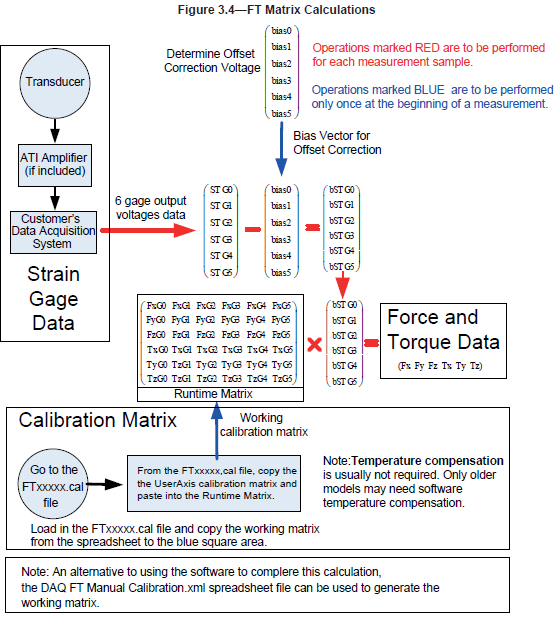
\includegraphics[width=0.9\textwidth]{load_calc.png}
	\label{fig:load_calc}
	\caption{Load calculation process}
\end{figure}

Additionally to this, gain correction factor is only required when a customer amplifier is being used. Refer to page 20 of the \hyperref{https://www.ati-ia.com/app_content/documents/9620-05-DAQ.pdf}{category}{name}{manual} for more information.

\section{Wiring and connecting to a DAQ}


There are two different wiring alternatives for the DAQ version of this sensor:

\begin{itemize}
	\item Differential connections to DAQ (\autoref{fig:diff_wiring}) 
	\item Single-ended connections to DAQ(\autoref{fig:se_wiring}) 
\end{itemize}

\begin{figure}[h!]
	\centering
	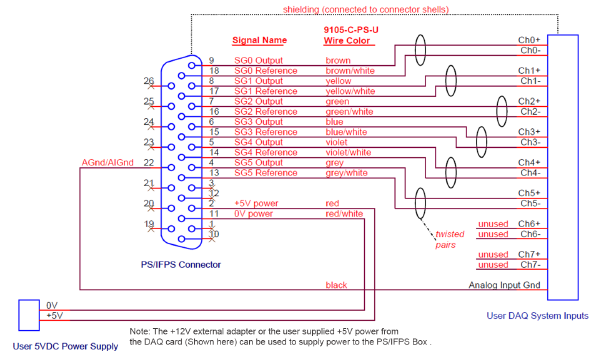
\includegraphics[width=0.7\textwidth]{diff_wiring.png}
	\caption{Differential wiring connections to data acquisition system (page 35 from \hyperref{https://www.ati-ia.com/app_content/documents/9620-05-DAQ.pdf}{category}{name}{9620-05-DAQ})}
	\label{fig:diff_wiring}
\end{figure}

\begin{figure}[h!]
	\centering
	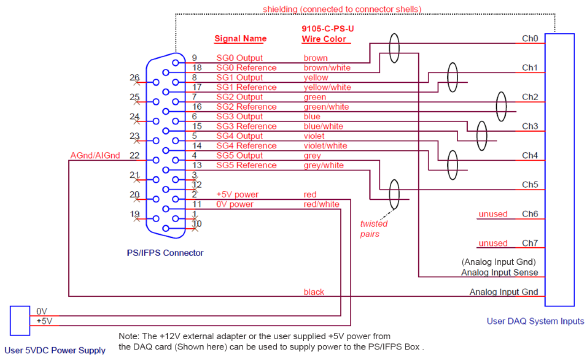
\includegraphics[width=0.7\textwidth]{se_wiring.png}
	\caption{Single-ended wiring connections to data acquisition system (page 36 from \hyperref{https://www.ati-ia.com/app_content/documents/9620-05-DAQ.pdf}{category}{name}{9620-05-DAQ})}
	\label{fig:se_wiring}
\end{figure}

A connection from the DAQ F/T's AGnd/AIGnd line to the data acquisition system’s analog input ground or analog ground is required in most cases.
This line allows the return of the small amount of current used by the data acquisition system. Noise can result if this current isn't returned via the AGnd/AIGnd path.
For best noise performance, the cabling from the PS/IFPS connector should be shielded and each strain gauge's signals in a twisted pair. The shielding should be connected to the PS/IFPS connector shell and to the shell of the data acquisition system’s connector. If the data acquisition system has no connector or its connector shell is electrically floating, then the shield at the PS/IPFS connector should be connected to the AGnd/AIGnd signal.

\subsection{Sampling}

For best performance in all applications (page 37 from \hyperref{https://www.ati-ia.com/app_content/documents/9620-05-DAQ.pdf}{category}{name}{9620-05-DAQ}),
the transducer electronics have bandwidth of 5kHz to 10kHz (depending on gain settings). This allows
collection of all transducer frequency content. Note: that to satisfy the Nyquist Theorem, the data needs
to be coupled at a rate greater than twice the highest frequency present, even if data at that frequency
is not preferred. The forces and torques will be sampled at that frequency, not having anything to do with the sampling rate of the data acquisition unit. 

The data acquisition unit on the other hand has a maximum aperture time of 400$\mu$s, meaning that's the smallest amount of time it needs for opening and reading from one channel. This aperture time is equivalent to an integration time of 0.02 PLC. The relationship between this two parameters is the following:

\begin{equation}
	\frac{0.02PLC}{50Hz (instrument power frequency)} = 400\mu s
\end{equation}

Using a differential wiring with 12 channels, we will need to multiply that aperture time by the number of channels:

\begin{equation}
	400\mu s \cdot 12 = 4800\mu s
\end{equation}

An aperture time of 4.8 ms is equivalent to a frequency of around 208 Hz. Rounding the aperture time to 5 ms per data volume (a vector containing one voltage value for each channel), we can obtain 10 measurements every 50 ms. 

\begin{figure}
	\centering
	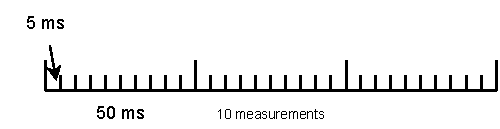
\includegraphics[width=0.8\textwidth]{sample_rate.pdf}
	\label{fig:sample_rate}
	\caption{Representation of trigger timer of 50 ms and 10 scans of }
\end{figure}
\subsection{Range}
As specified in the ATI \hyperref{https://www.ati-ia.com/products/ft/ft_models.aspx?id=mini40}{category}{name}{site}, the range of the sensor for the calibration US-20-40 is the following defined as the average of the worst and best case
scenarios:

\begin{table}[h!]
	\centering
	\caption{Range values in imperial and metric systems\label{tab:range}}
	\begin{tabular}{||c | c | c | c||} 
		\hline
		Fx, Fy & Fz & Tx,Ty & Tz \\ [0.5ex] 
		\hline\hline
		$\pm$ 20 lbf & $\pm$ 60 lbf & $\pm$ 40 lbf-in & $\pm$ 40 lbf-in\\ 
		\hline
		$\pm$ 88.9644 N & $\pm$ 266.893 N & $\pm$ 4.51939 N-m & $\pm$ 4.51939 N-m \\
		\hline
		
	\end{tabular}
\end{table}

\subsection{Resolution}
As specified in the ATI \hyperref{https://www.ati-ia.com/products/ft/ft_models.aspx?id=mini40}{category}{name}{site}, the resolution of the sensor for the calibration US-20-40 is the following defined as the average of the worst and best case
scenarios:

\begin{table}[h!]
	\centering
	\caption{Resolution values in imperial and metric systems\label{tab:resolution}}
	\begin{tabular}{||c | c | c | c||} 
		\hline
		Fx, Fy & Fz & Tx,Ty & Tz \\ [0.5ex] 
		\hline\hline
		1/200 lbf & 1/100 lbf & 1/200 lbf-in & 1/200 lbf-in\\ 
		\hline
		0.022241108 N & 0.0444822 N & 0.000564924 N-m & 0.000564924 N-m \\
		\hline
	\end{tabular}
\end{table}

\subsection{Sensitivity and output range and resolution voltages}

From page 54 of the transducer \href{https://www.ati-ia.com/app_content/documents/9620-05-Transducer%20Section.pdf}{manual}, we can obtain the analog $\pm$ 10 V sensitivity. Using the data from tables \ref{tab:range} and \ref{tab:resolution}, we can obtain the following table:

\begin{table}[h!]
	\centering
	\caption{Sensitivity, range and resolution outputs voltages\label{tab:sensit} (imperial system)}
	\begin{tabular}{||c | c | c | c ||} 
		\hline
		 & Fx, Fy & Fz & Tx,Ty,Tz \\ [0.5ex] 
		\hline\hline
		Analog $\pm$ 10V sensitivity & 2 lbf/V & 6 lbf/V & 4 lbf-in/V\\ 
		\hline
		Range [V] & $\pm$ 10 & $\pm$ 10 & $\pm$ 10 \\
		\hline
		Resolution [V] & 1/400 & 1/600 & 1/800 \\
		\hline
	\end{tabular}
\end{table}

The minimum voltage that the DAQ must be able to measure is 1/800 V = 1.25 mV. The range must be $\pm$ 10 V.

Just for clarity purposes, \autoref{tab:sensit} in metric system would be as follows:

\begin{table}[h!]
	\centering
	\caption{Sensitivity, range and resolution outputs voltages\label{tab:sensit2} (metric system)}
	\begin{tabular}{||c | c | c | c ||} 
		\hline
		& Fx, Fy & Fz & Tx,Ty,Tz \\ [0.5ex] 
		\hline\hline
		Analog $\pm$ 10V sensitivity & 8.89644 N/V & 26.6893 N/V & 17.7929 N/V\\ 
		\hline
		Range [V] & $\pm$ 10 & $\pm$ 10 & $\pm$ 10 \\
		\hline
		Resolution [V] & 1/400 & 1/600 & 1/800 \\
		\hline
	\end{tabular}
\end{table}


\section{Keysight 34970A connection to PC}
The connection is made via a GPIB‑USB‑HS cable. The GPIB‑USB‑HS is an IEEE 488 controller device for computers with USB slots. The GPIB‑USB‑HS achieves maximum IEEE 488.2 performance. The exact model can be found in \hyperref{https://www.amazon.com/Kanonaki-GPIB-USB-HS-Interface-Adapter-Controller/dp/B07Q84XJJF}{category}{name}{Amazon}. The differences with the \hyperref{https://www.newark.com/ni/780570-01/gpib-usb-hs-gpib-control-device/dp/14AJ5119}{category}{name}{original} true version of this device are not the sxope of this document. 

There are various manuals for this DAQ. The most helpful one containing command examples is the \href{https://documentation.help/Keysight-34970A-34972A/documentation.pdf}{Keysight 34970A/34972A Command Reference Manual}. From this manual, the information from the following section was found.

\subsection{Important commands}

\textbf{ROUT:SCAN} : This command selects the channels to be included in the scan list. This command is used in conjunction with the CONFigure commands to set up an automated scan. To start the scan, use the INITiate or READ? command.

\textbf{INStrument:DMM} : This command disables or enables the internal digital multimeter. When you change the state of the internal DMM, the instrument issues a Factory Reset (*RST command).

\textbf{TRIGger:SOURce} : Select the trigger source to control the onset of each sweep through the scan list (a sweep is one pass through the scan list). The instrument will accept a software (bus) command, an immediate (continuous) scan trigger, an external TTL trigger pulse, an alarm-initiated action, or an internally paced timer. Usually used: TIMer = Internally paced timer trigger.

\textbf{TRIGger:TIMer} : This command sets the trigger-to-trigger interval (in seconds) for measurements on the channels in the present scan list. This command defines the time from the start of one trigger to the start of the next trigger, up to the specified trigger count (see TRIGger:COUNt command). A number from 0 seconds to 359,999 with 1 ms resolution. Note that 359,999 seconds is one second less than one hundred hours.


\begin{figure}[h!]
	\centering
	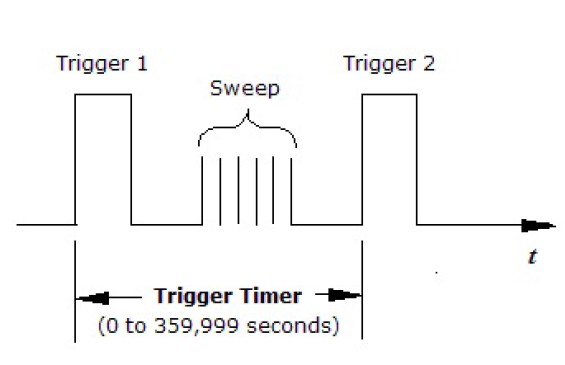
\includegraphics[width=0.7\textwidth]{trigger_timer.png}
	\label{fig:trigger_timer}
	\caption{Trigger timer}
\end{figure}

\begin{figure}[h!]
	\centering
	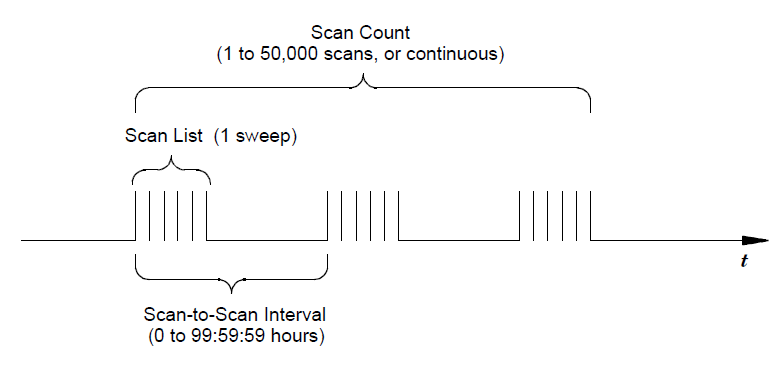
\includegraphics[width=0.7\textwidth]{trigger_timer2.png}
	\label{fig:trigger_timer2}
	\caption{Trigger timer from hewlett packard manual}
\end{figure}



\textbf{TRIGger:COUNt}: This command specifies the number of times to sweep through the scan list. A sweep is one pass through the scan list. The scan stops when the number of specified sweeps has occurred. An integer from 1 to 50,000 triggers, or continuous (INFinity).

\textbf{INITiate} : This command changes the state of the triggering system from the ``idle" state to the ``wait-for-trigger" state. Scanning will begin when the specified trigger conditions are satisfied following the receipt of the INITiate command. Readings are stored in the instrument's internal reading memory. Note that the INITiate command also clears the previous set of readings from memory.
If a scan list is currently defined (see ROUTe:SCAN command), the INITiate command performs a scan of the specified channels.
Storing readings in memory using the INITiate command is generally faster than sending readings to memory using the READ? command. The INITiate command is also an "overlapped" command. This means that after executing the INITiate command, you can send other commands that do not affect the measurements.
You can store up to 50,000 readings in memory and all readings are automatically time stamped. If memory overflows, the new readings will overwrite the first (oldest) readings stored; the most recent readings are always preserved.
For scanning measurements using the multiplexer modules, an error is generated if the internal DMM is disabled.
To retrieve the readings from memory, use the FETCh? command.
The readings are not erased from memory when you read them.
You can send the command multiple times to retrieve the same data in reading memory.

\textbf{FETCh}: This command transfers readings stored in non-volatile memory to the instrument's output buffer, where you can read them into your computer. The readings stored in memory are not erased when you read them with FETCh?.

\textbf{VOLT:DC:APERTURE} : This command enables the aperture mode and sets the integration time in seconds (called aperture time) for DC voltage measurements on the specified channels.


\section{LabView}

For LabView, a calibration file has to be loaded inside the VI. Use the file FT17838.cal and choose desired units. May not work well when using single-ended connection. In that case, use the matrices provided in ATImatrices.m under the MATLAB/Scripts folder.

\subsection{Keysight 34970A}

LabView offers two main ways of interacting with the Keysight 34970A DAQ:

\begin{itemize}
	\item General purpose Virtual Instrument Software Architecture (VISA) blocks.NI-VISA is an API that provides a programming interface to control Ethernet/LXI, GPIB, serial, USB, PXI, and VXI instruments in NI application development environments like LabVIEW, LabWindows/CVI, and Measurement Studio. The API is installed through the NI-VISA driver \cite{NIVISA}.
	\item Agilent Technologies / Keysight Technologies 34970A \hyperref{http://sine.ni.com/apps/utf8/niid_web_display.model_page?p_model_id=5547}{category}{name}{drivers}. These block are based on the VISA blocks but offer a more user-friendly approach to configuring the instrument as well as reading data from it. 
\end{itemize}

The \hyperref{https://github.com/IrisDuMutel/ATIMini40_software/tree/master/LabView}{cat1}{visa}{example}  provided in this repository uses generic VISA blocks. In \autoref{fig:labview_block}, the block diagram of the VI can be seen:

\begin{figure}[!h]
	\centering
	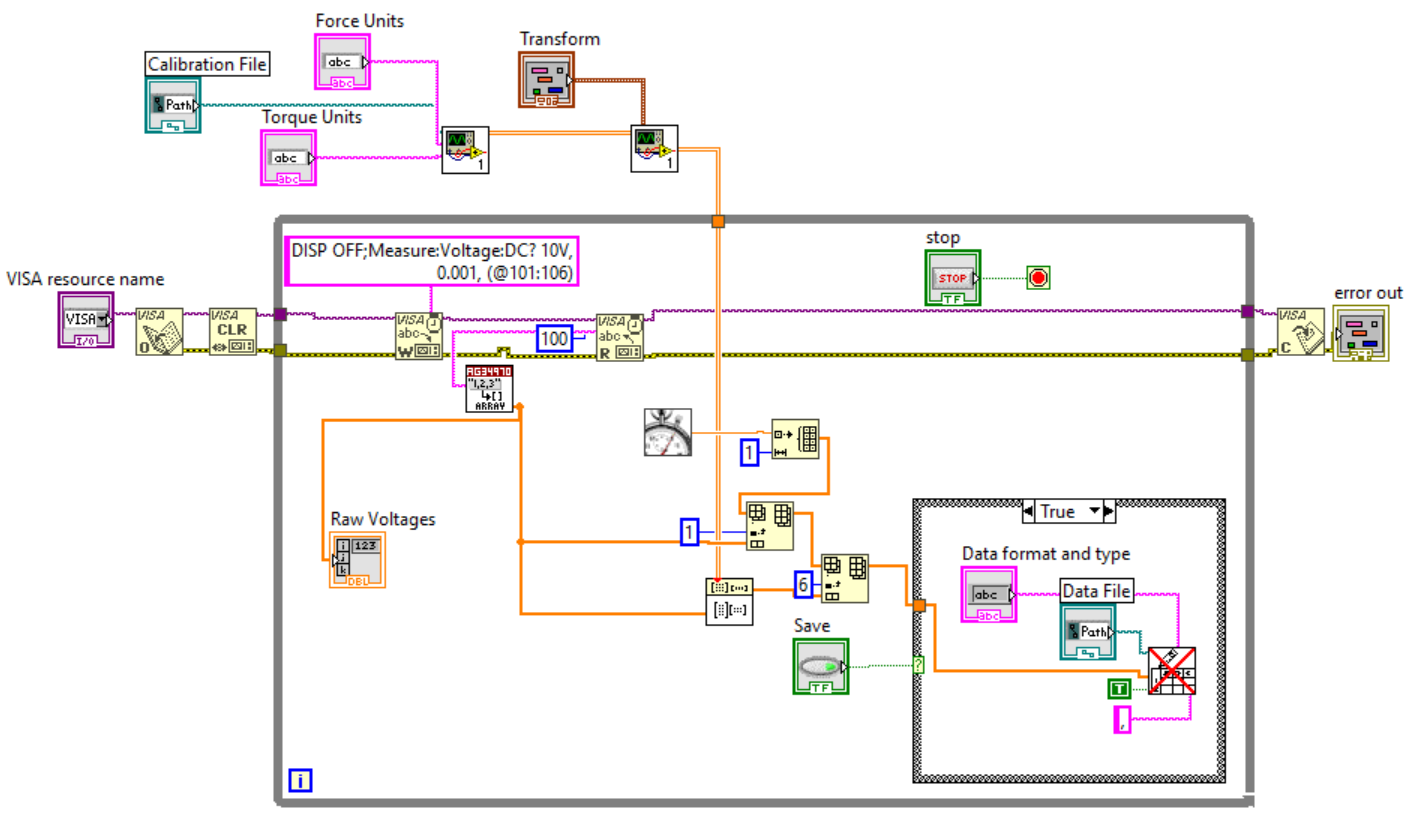
\includegraphics[width=0.9\textwidth]{labview_block.png}
	\caption{LabView block diagram}
	\label{fig:labview_block}
\end{figure}

Inside the while loop, the write and read blocks are interacting with the instrument. Every iteration, the \textit{write} block sends the following commands to the DAQ:

\begin{itemize}
	\item DISP OFF: This command turns off the display of the external instrument. This speeds up the sampling process.
	\item MEASure:VOLTage:DC? 10V, 0.001, (@101:106): The first part of the command 'MEASure:VOLTage:DC$?$` is requesting the measurement of the voltage. The question mark indicates a query command. The two numbers following such query are the \textit{range} and the \textit{resolution}, respectively. There are alternative values for these parameters. See more in pages 211 to 217 from the \hyperref{https://www.manualsbase.com/manual/439362/switch/hp_(hewlett-packard)/hp_34970a/}{category}{name}{manual}.
\end{itemize}

\subsection{NI USB 6008}

Using the VI provided by the \hyperref{https://www.ati-ia.com/products/ft/software/daq_software.aspx}{category}{name}{DAQ software download page} from ATI.


\section{Python}

Using \hyperref{https://www.qt.io/product/development-tools}{category}{name}{Qt creator}, a base interface was created to interact with all python codes (see \autoref{fig:NIUSB6008_GUI}). Since the final choice for the DAQ was the NI USB 6008, the interface has been adapted to the configuration parameters of this specific device.

There are several ways of creating a multi-channel analog reading software using Qt and the NI-DAQmx python libraries \cite{goncalo}:

\begin{itemize}
	\item \textbf{NI Callback functions}: 
	\item \textbf{\hyperref{https://doc.qt.io/qt-6/qtimer.html}{category}{name}{QTimers}} $\leftarrow$ used in this project for ATI Mini40 and NI USB 6008 DAQ.
	\item \textbf{\hyperref{https://realpython.com/intro-to-python-threading/}{category}{name}{Python Threads}} :
\end{itemize}


Please, visit \hyperref{http://engredu.com/2023/07/29/ni-acquisition-strategies/}{category}{name}{ENGedu} for fantastic code examples and references using these methods.

\begin{figure}[h!]
	\centering
	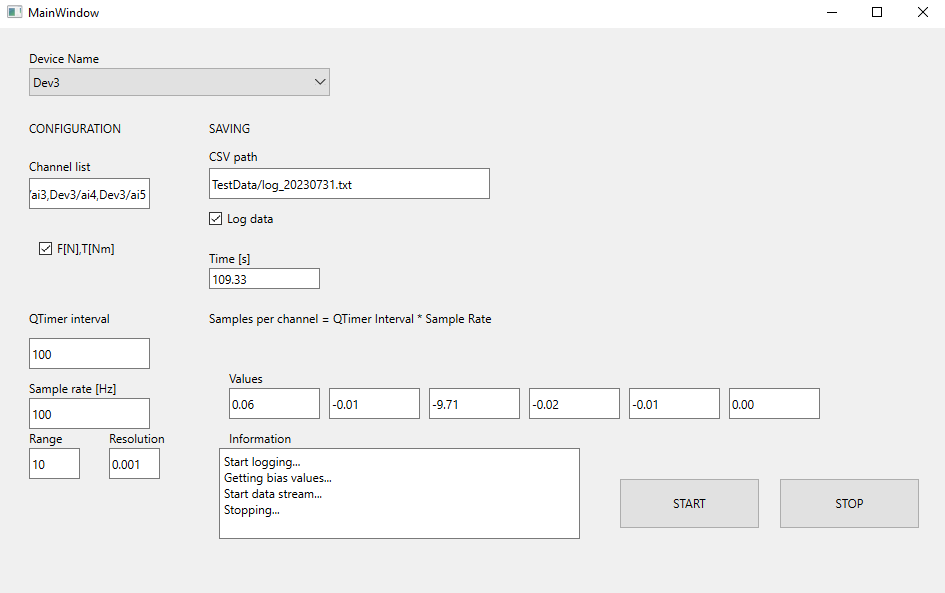
\includegraphics[width=0.7\textwidth]{NIUSB6008_GUI.png}
	\caption{Qt interface for NI USB 6008 Data Acquisition Unit}
	\label{fig:NIUSB6008_GUI}
\end{figure}


\subsection{Keysight 34790A}

Using \hyperref{https://pyvisa.readthedocs.io/en/latest/index.html}{name}{category}{PyVisa} python libraries.

\subsection{NI USB 6008 DAQ}

Using \hyperref{https://nidaqmx-python.readthedocs.io/en/latest/}{name}{cat}{NI-DAQmx} python libraries.

\begin{figure}[h!]
	\begin{subfigure}{.5\textwidth}
		\centering
		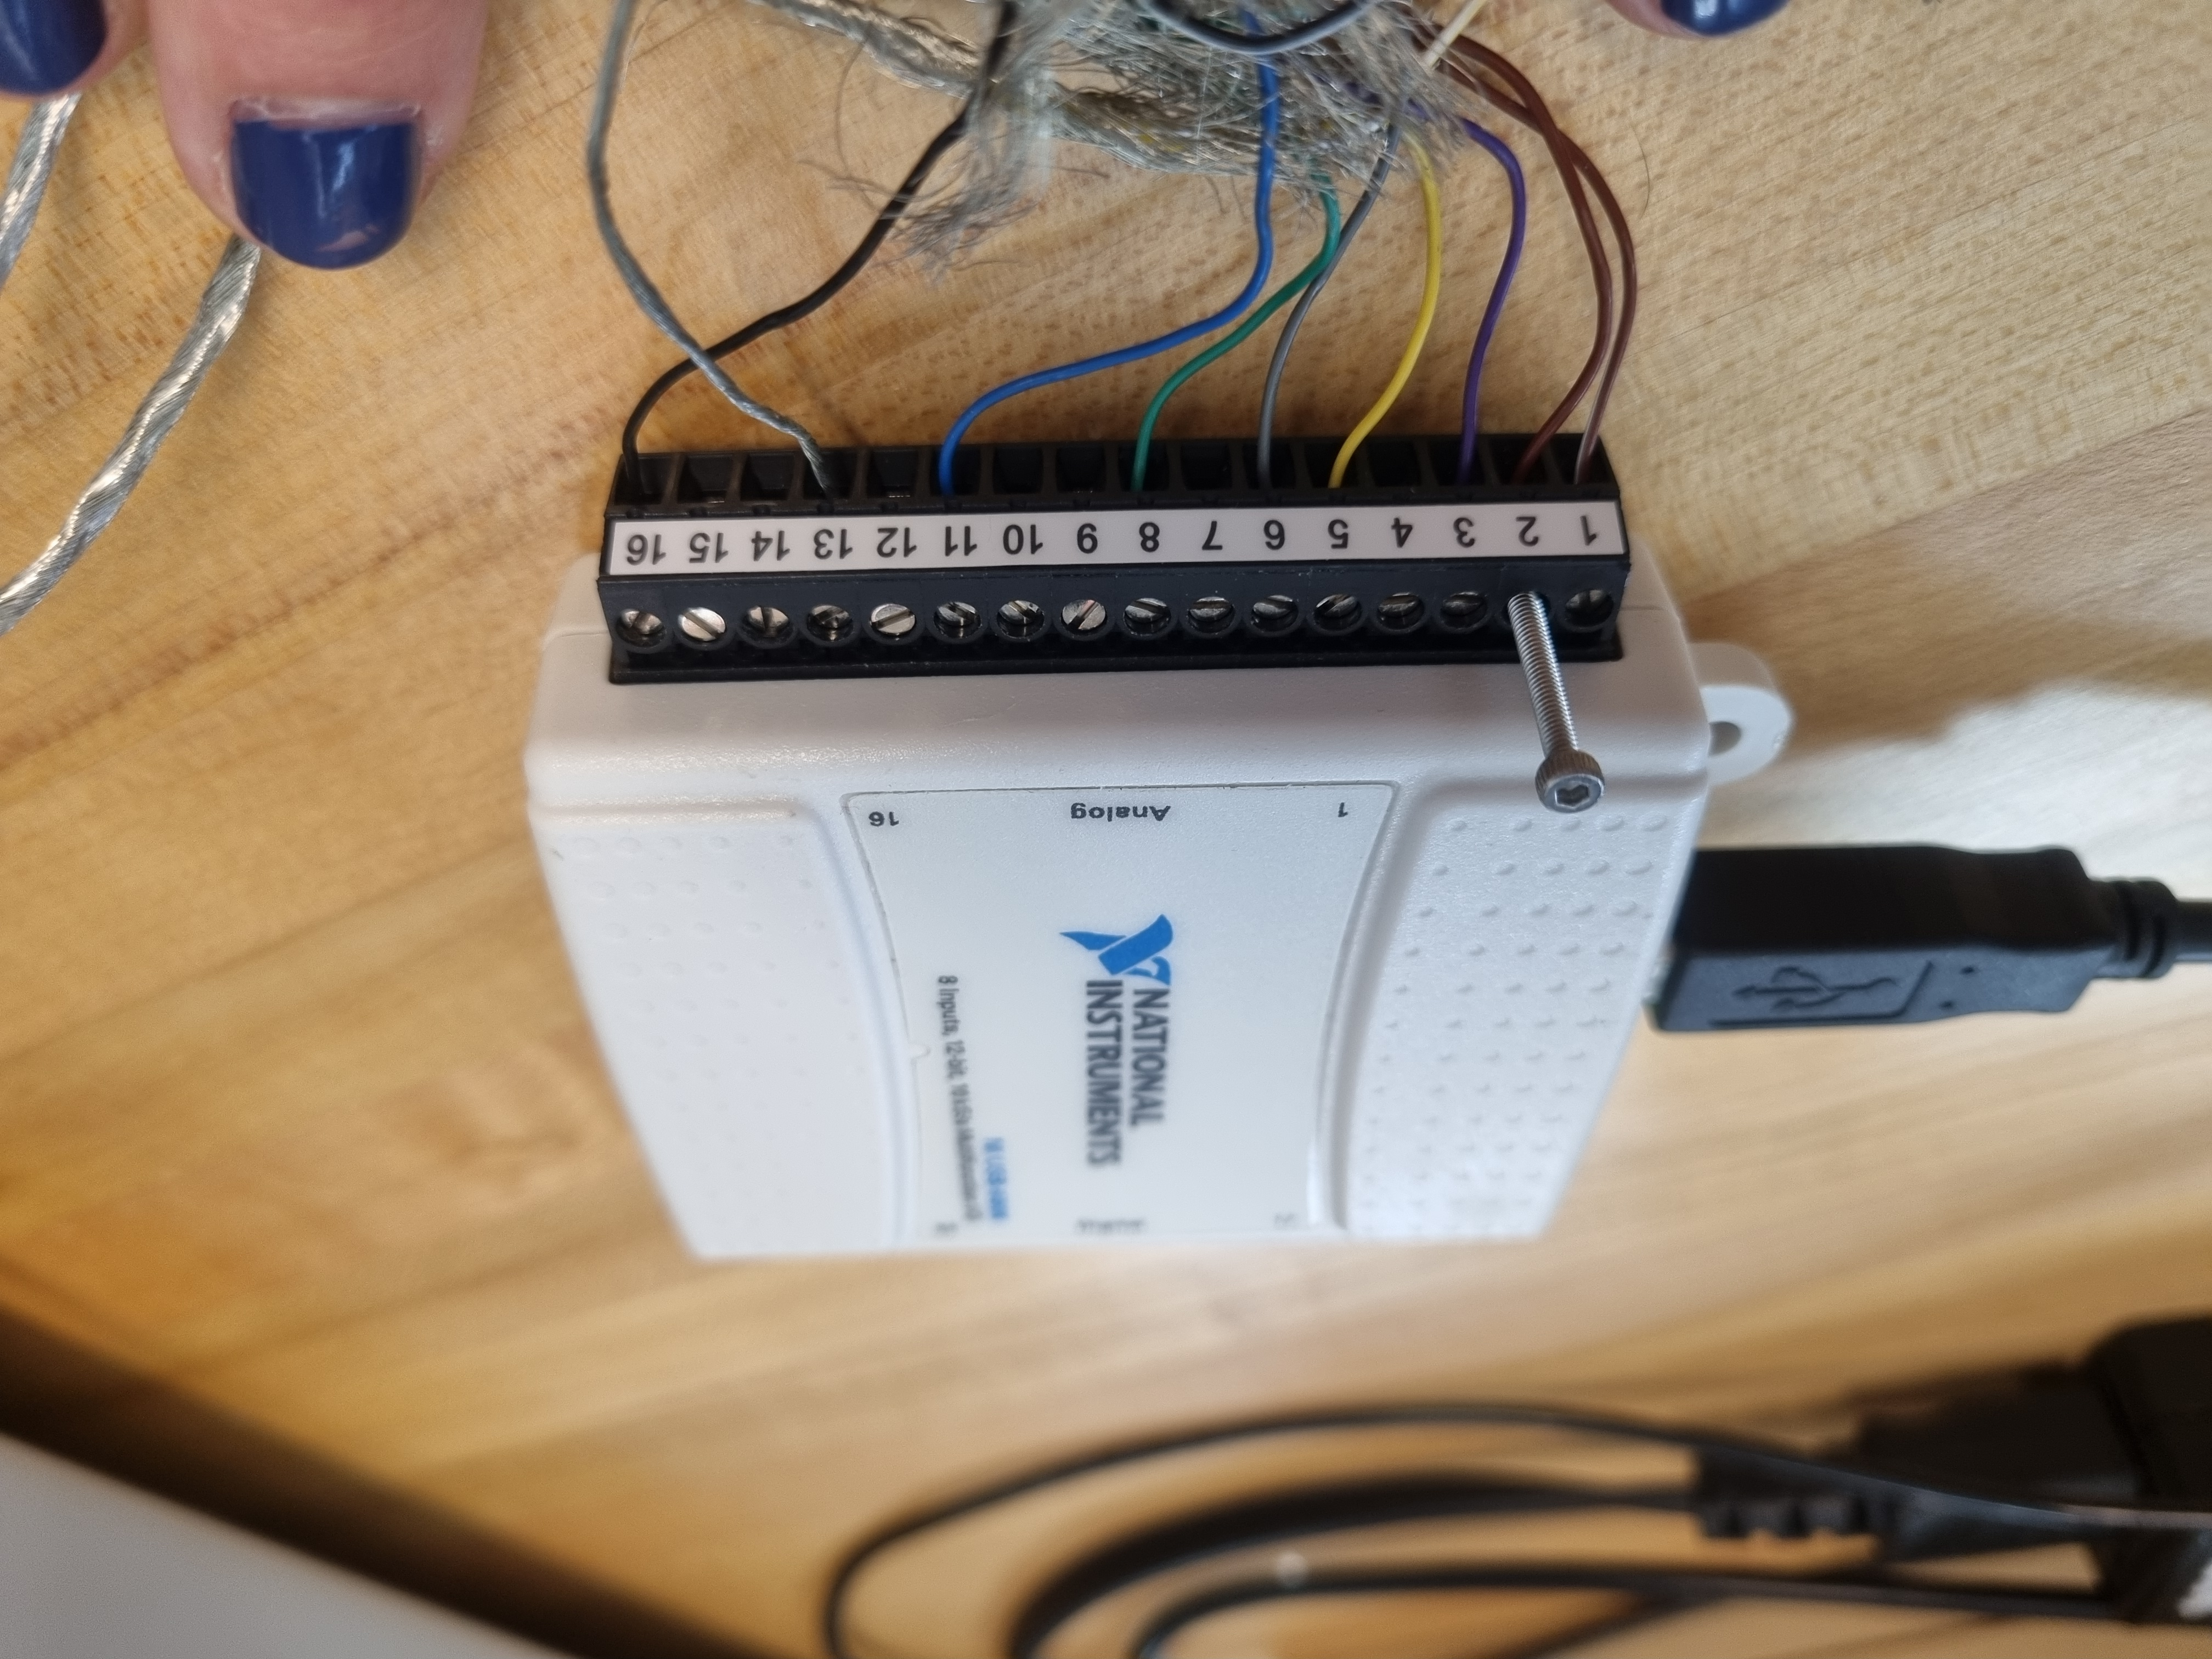
\includegraphics[width=0.7\textwidth,angle=180]{NIUSB6008_ATIMini40Connection.jpg}
		\caption{Single-ended connection with only brown-white reference cable grounded}
		\label{fig:NIUSB6008_ATIMini40Connection}
	\end{subfigure}%
	\begin{subfigure}{.5\textwidth}
		\centering
		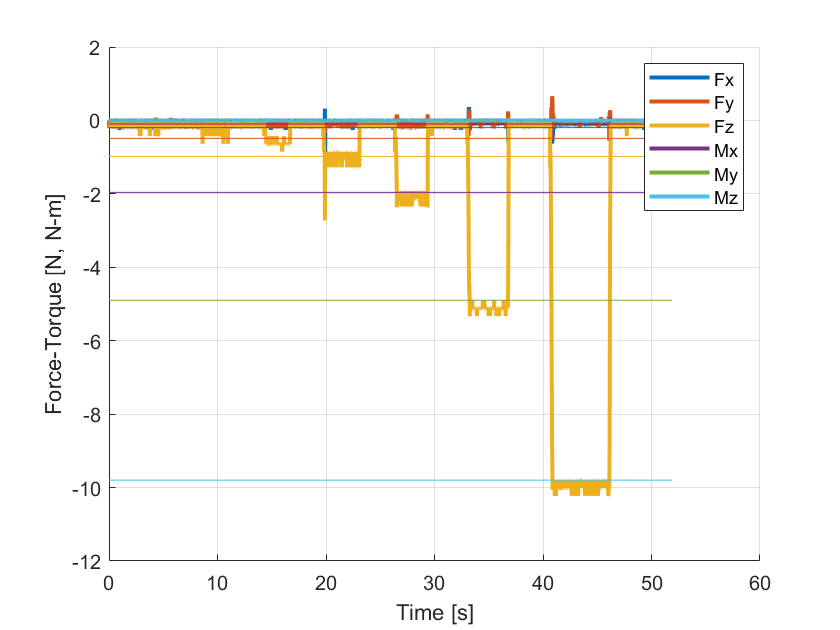
\includegraphics[width=.8\linewidth]{Forces_check50Hz.png}
		\caption{Fz test check}
		\label{fig:Forces_check50Hz}
	\end{subfigure}
	\caption{Single-ended connection results with non-connected references}
	\label{fig:test1}
\end{figure} 

\begin{figure}[h!]
	\begin{subfigure}{.5\textwidth}
		\centering
		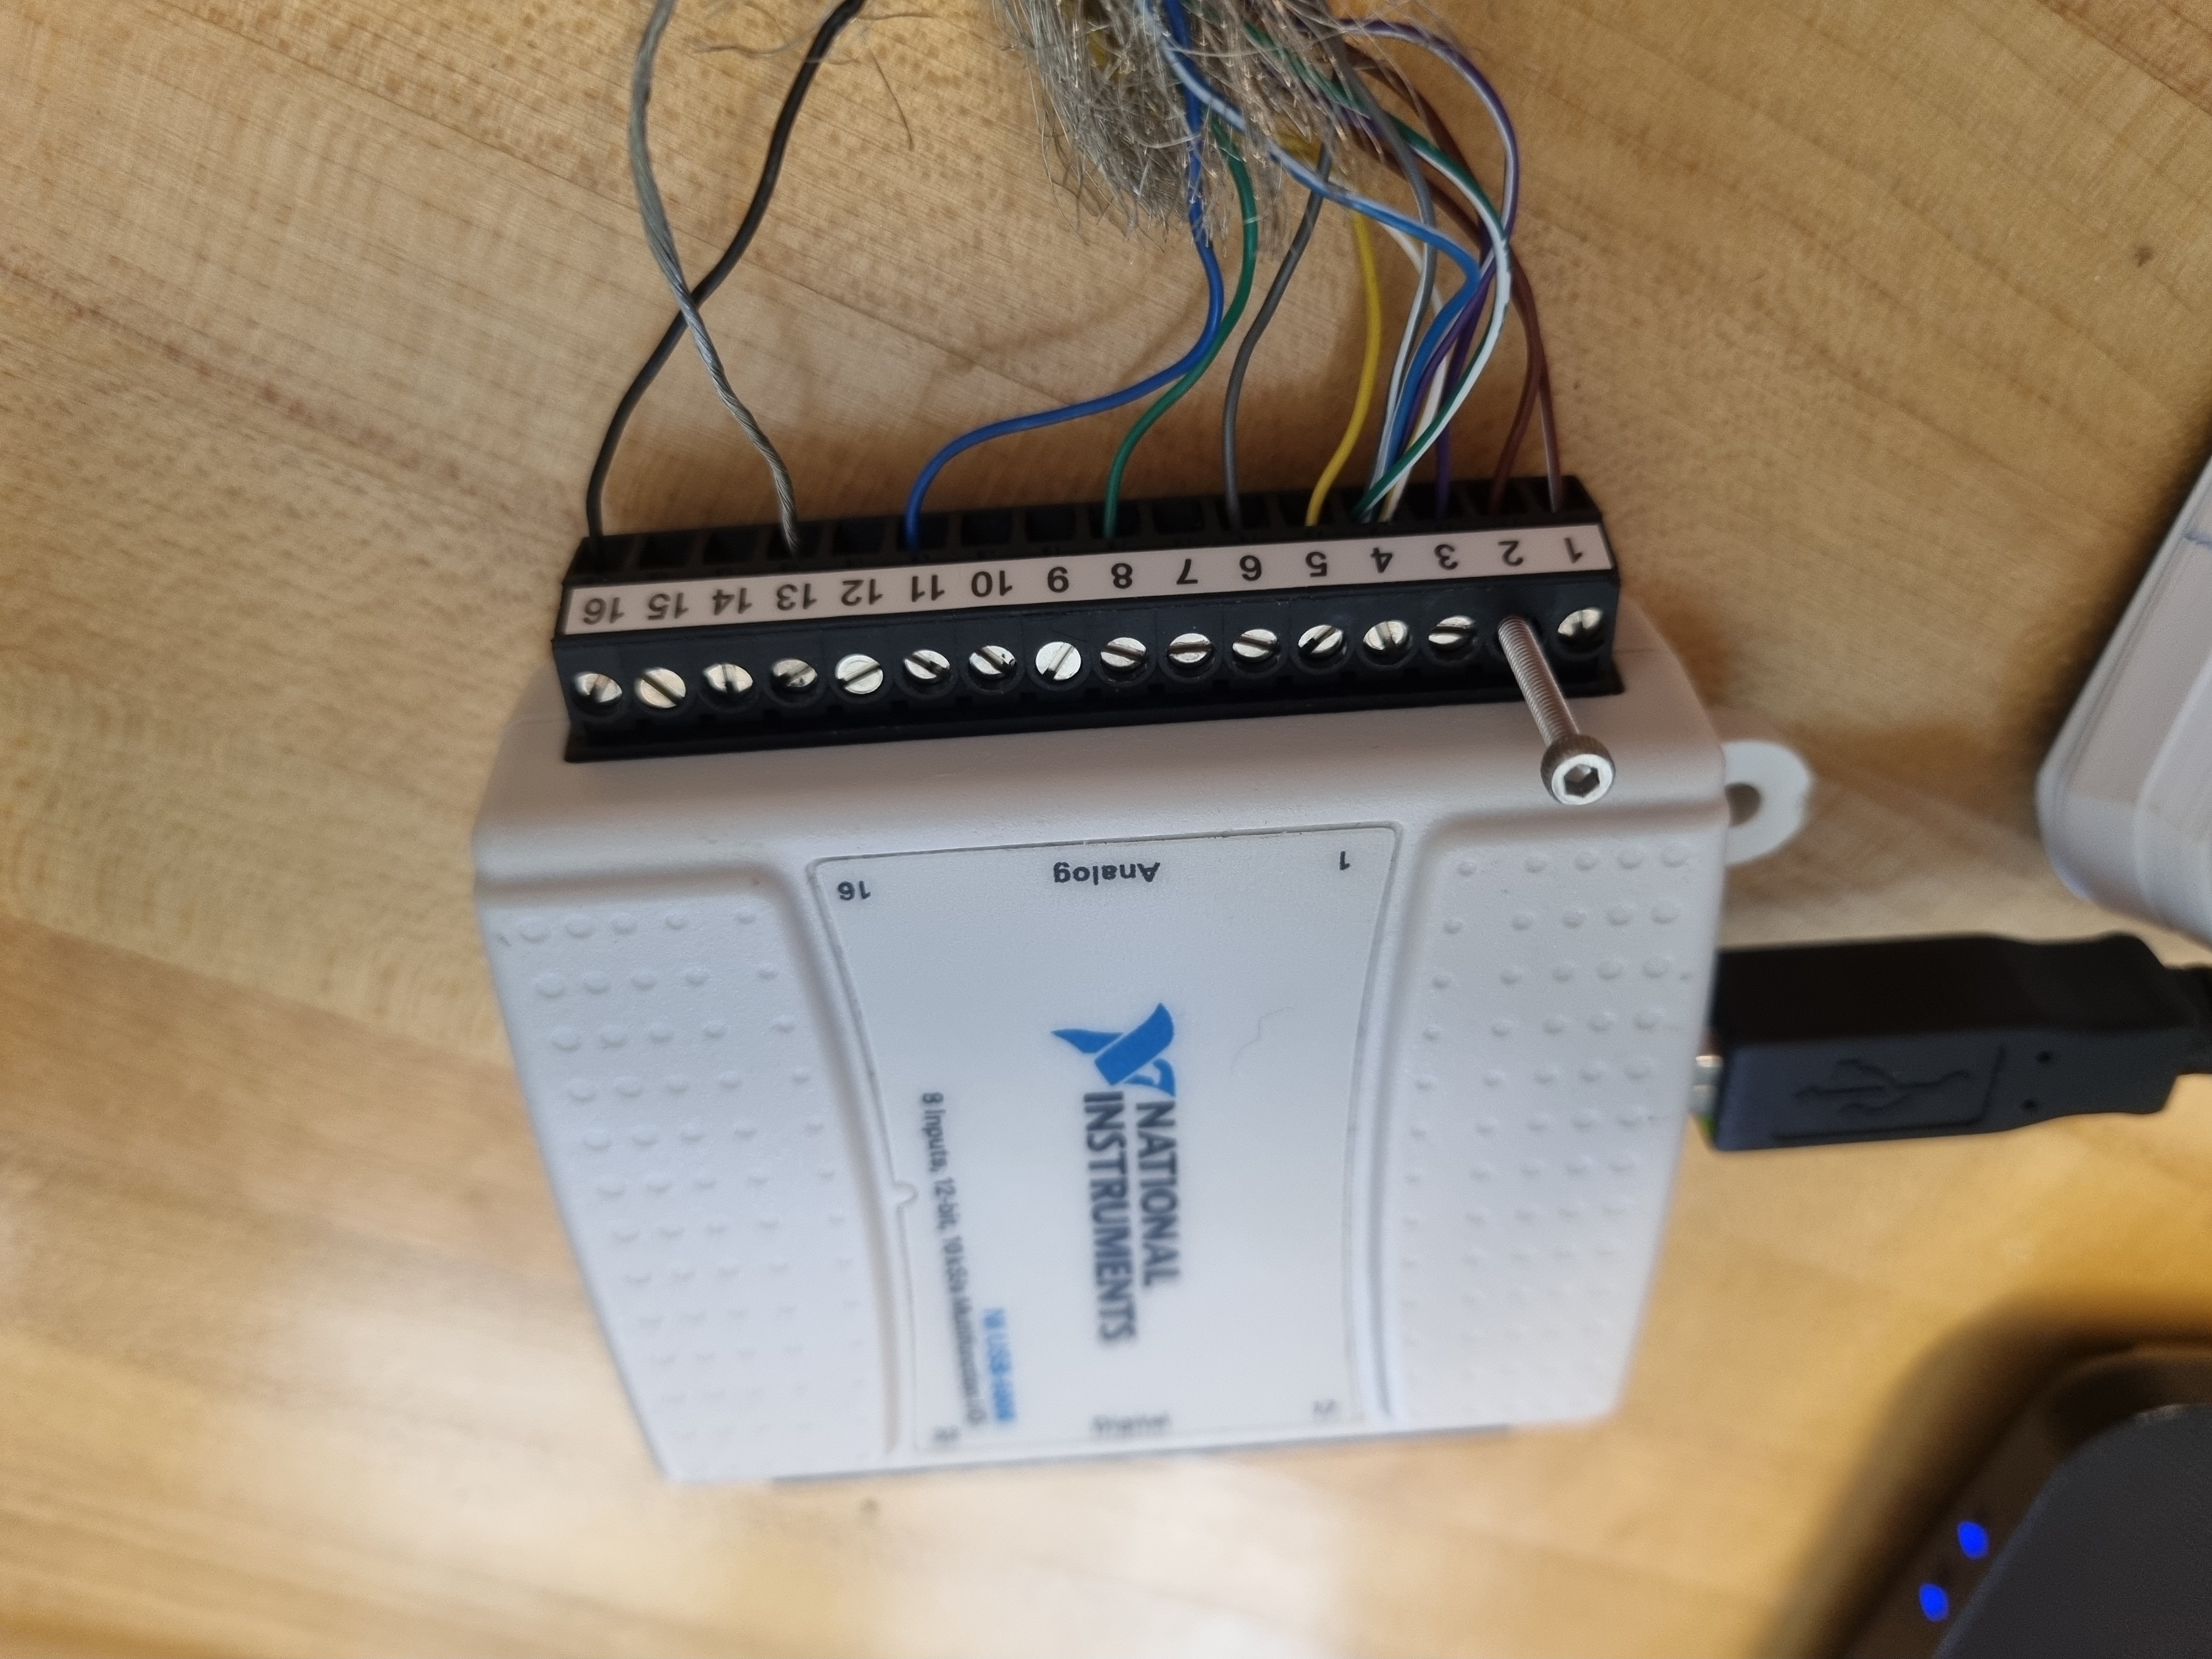
\includegraphics[width=0.7\textwidth,angle=180]{NIUSB6008_ATIMini40Connection_grounded.jpg}
		\caption{Single-ended connection with all reference cables grounded}
		\label{fig:NIUSB6008_ATIMini40Connection}
	\end{subfigure}%
	\begin{subfigure}{.5\textwidth}
		\centering
		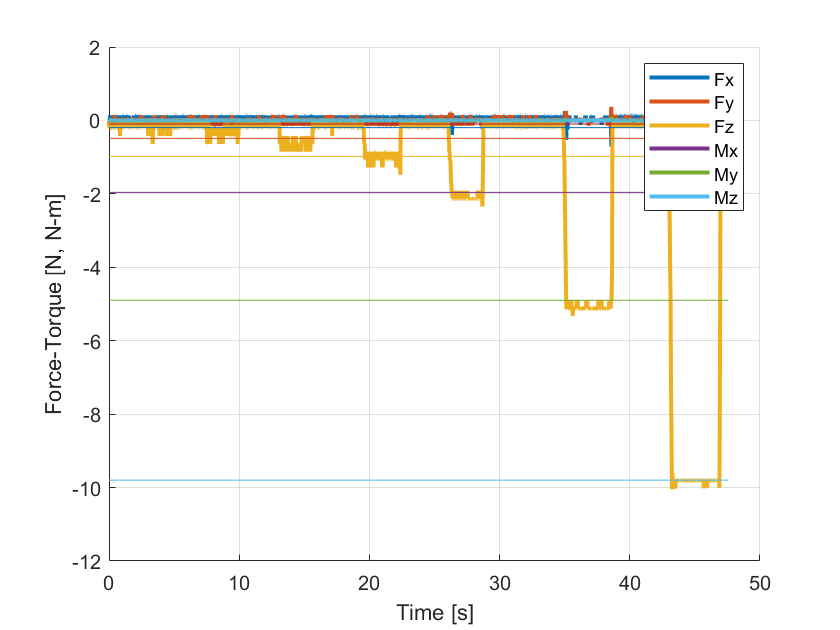
\includegraphics[width=.8\linewidth]{Forces_check50Hz_grounded.png}
		\caption{Fz test check}
		\label{fig:Forces_check50Hz_grounded}
	\end{subfigure}
	\caption{Single-ended connection results with grounded references}
	\label{fig:test2}
\end{figure}


The sampling frequency is chosen by the user. The default value is 150 Hz. In this case, being a high frequency, the Qtimer that is in charge of refreshing the GUI and in control of the python process needs to have a not so fast frequency. A QTimer of 500 ms is chosen as default. Th relationship between these two frequecies result in the following equation:

\begin{equation}
	Samples\hspace{1mm}per\hspace{1mm}channel = Desired\hspace{1mm}frequency[Hz] \cdot QTimer[s]
\end{equation}

In the case of this application, six channels are required. Using the default values, a total of 75 samples per channel is obtained.

To log data into a \textit{.txt} file, write the name of the desired file in the textbox and then check the \textit{log data} checkbox (see \autoref{fig:NIUSB6008_GUI}).


\section{SICK WLA16 Photoelectric sensors}

The \hyperref{https://www.sick.com/us/en/photoelectric-sensors/photoelectric-sensors/w16/wla16p-24162100a00/p/p512654}{sensors}{SICK}{SICK photoelectric sensors} have been chosen for this application as they have proven their applicability in UAV related research topics in the past \cite{Scanavino2021}. It has to be powered with 10 V to 20 V. For more specifications regarding the power of the sensor, see the \hyperref{https://cdn.sick.com/media/pdf/4/54/654/dataSheet_WLA16P-24162100A00_1218660_en.pdf}{category}{name}{manual}.

The connection type is as in \autoref{fig:SICKpins}:

\begin{figure}[h!]
	\begin{subfigure}{.5\textwidth}
		\centering
		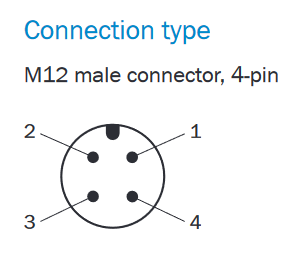
\includegraphics[width=0.5\textwidth]{SICKpins1.png}
		\label{fig:SICKpins2}
	\end{subfigure}%
	\begin{subfigure}{.5\textwidth}
		\centering
		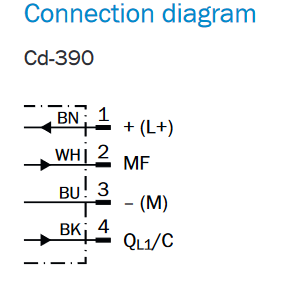
\includegraphics[width=.5\linewidth]{SICKpins2.png}
		\label{fig:SICKpins2}
	\end{subfigure}
	\caption{SICK WLA16 Photoelectric sensors pinout}
	\label{fig:SICKpins}
\end{figure} 

These sensors have four cables which have the following fucntionality:
\begin{itemize}
	\item Brown (pin 1): Positive power input.
	\item White (pin 2): Digital output. When and object is present between the sensor and the reflector, the signal is high. If not, signal is low.
	\item Blue (pin 3): GND 	
	\item Black (pin 4): Digital output. When an object is present between the sensor and the reflector, the signal is low. If not, signal is high.
\end{itemize}

The arduino connection to be used with the \textit{sensor\_analog.ino} script are as in \autoref{fig:sick_arduino_analog}:

\begin{figure}
	\centering
	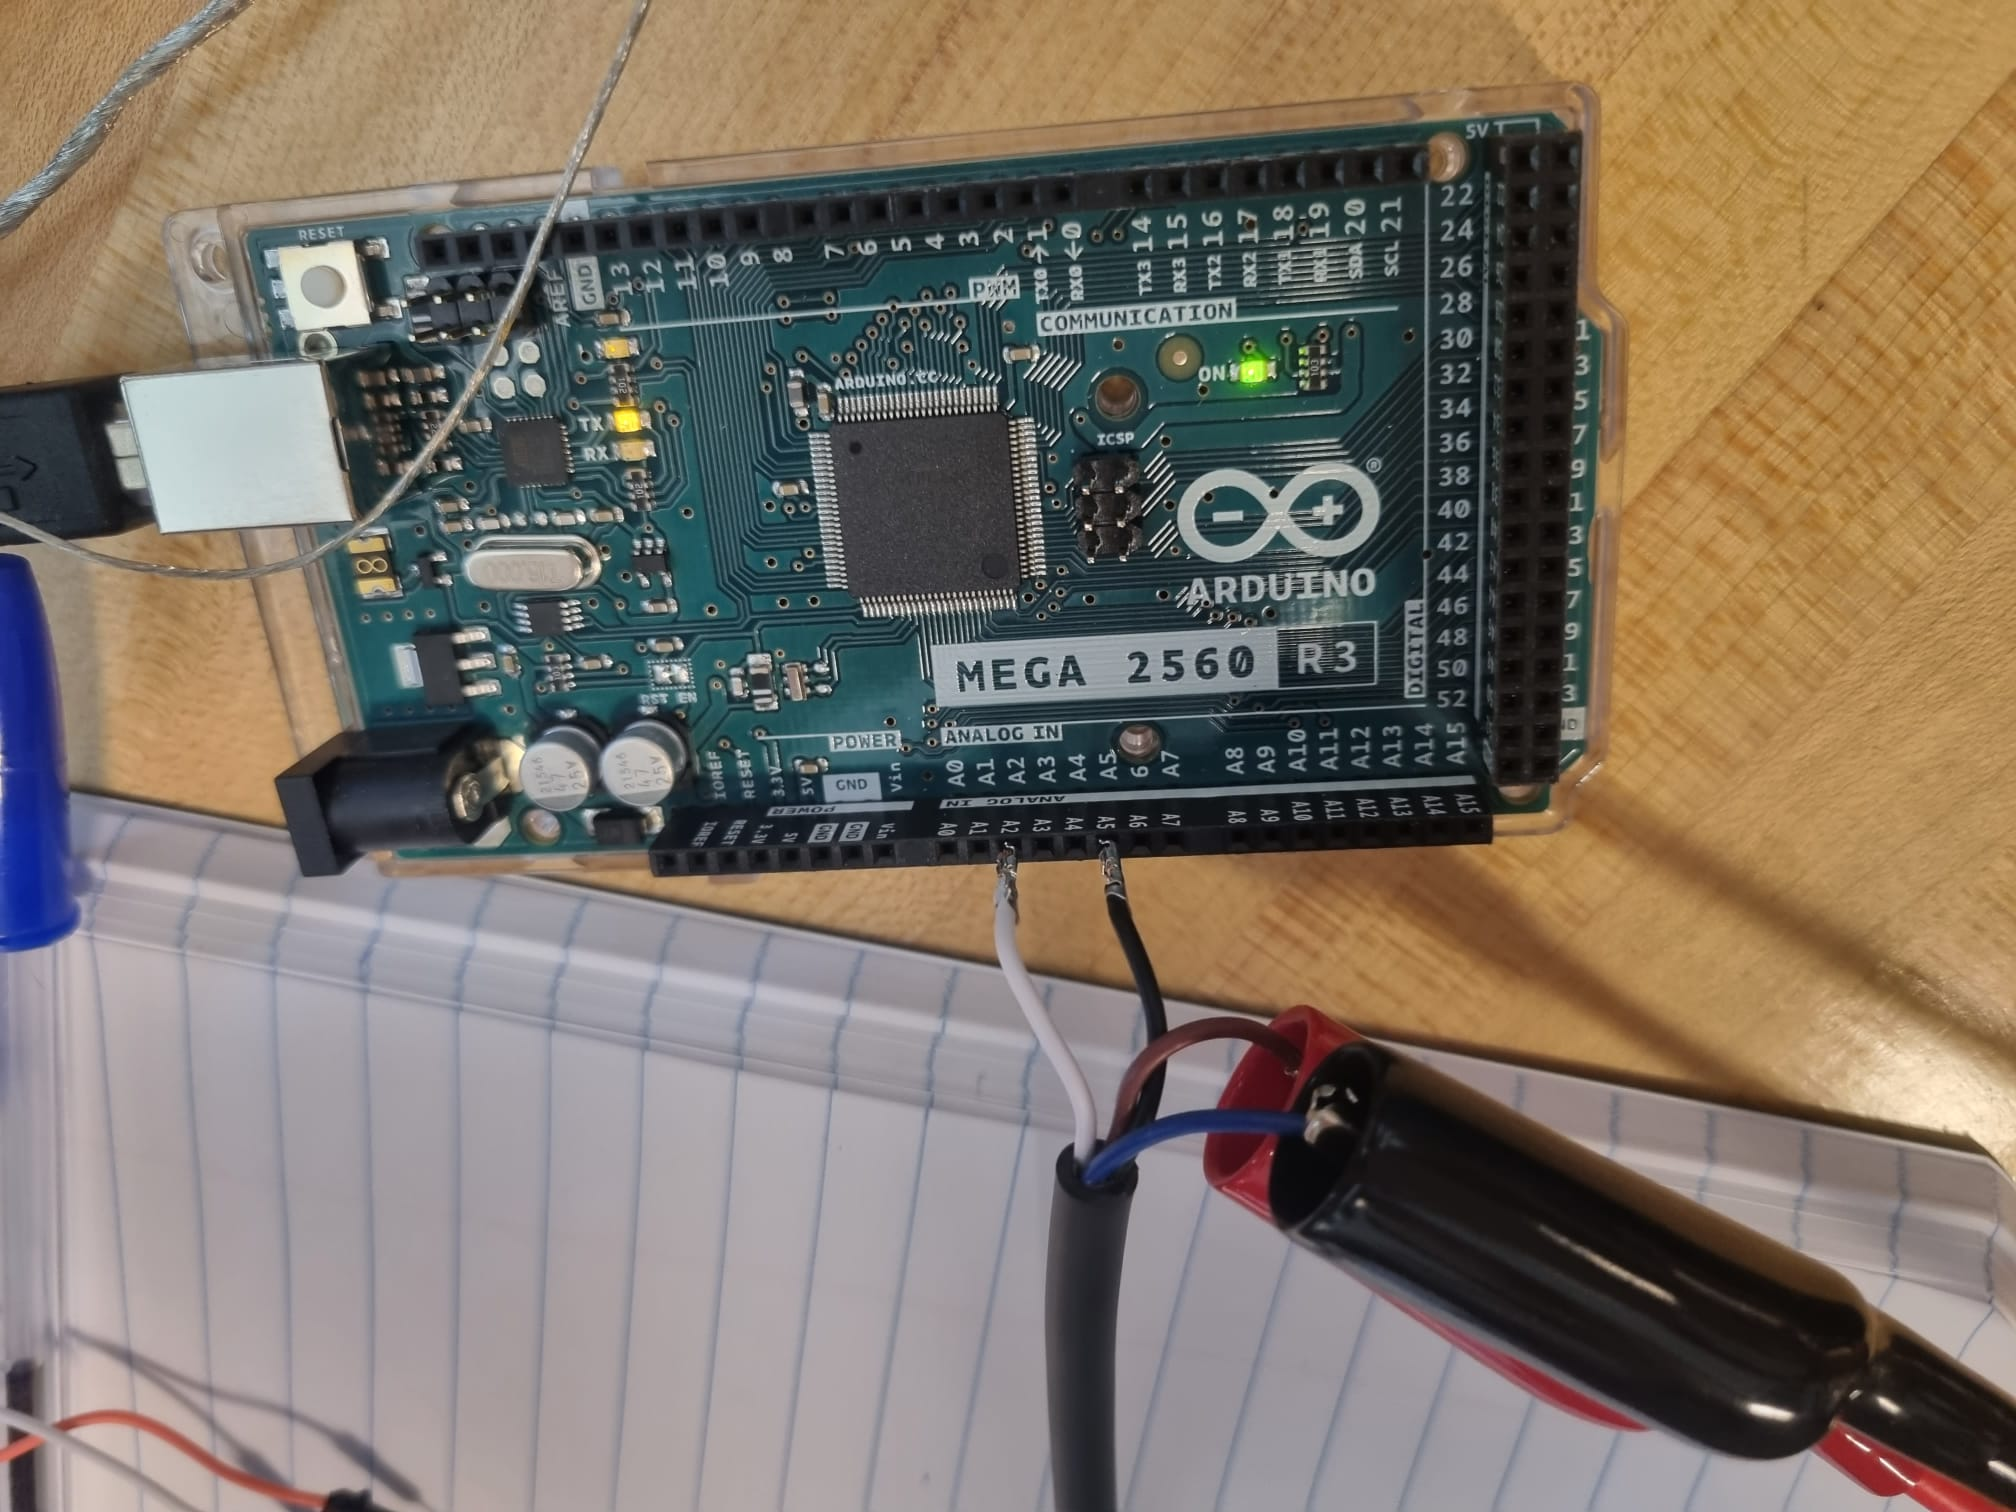
\includegraphics[width=0.5\textwidth,angle=180]{SICK_arduino.jpg}
	\caption{SICK sensor analog connection to arduino mega 2560 R3}
	\label{fig:sick_arduino_analog}
\end{figure}

\begin{figure}[h!]
	\centering
	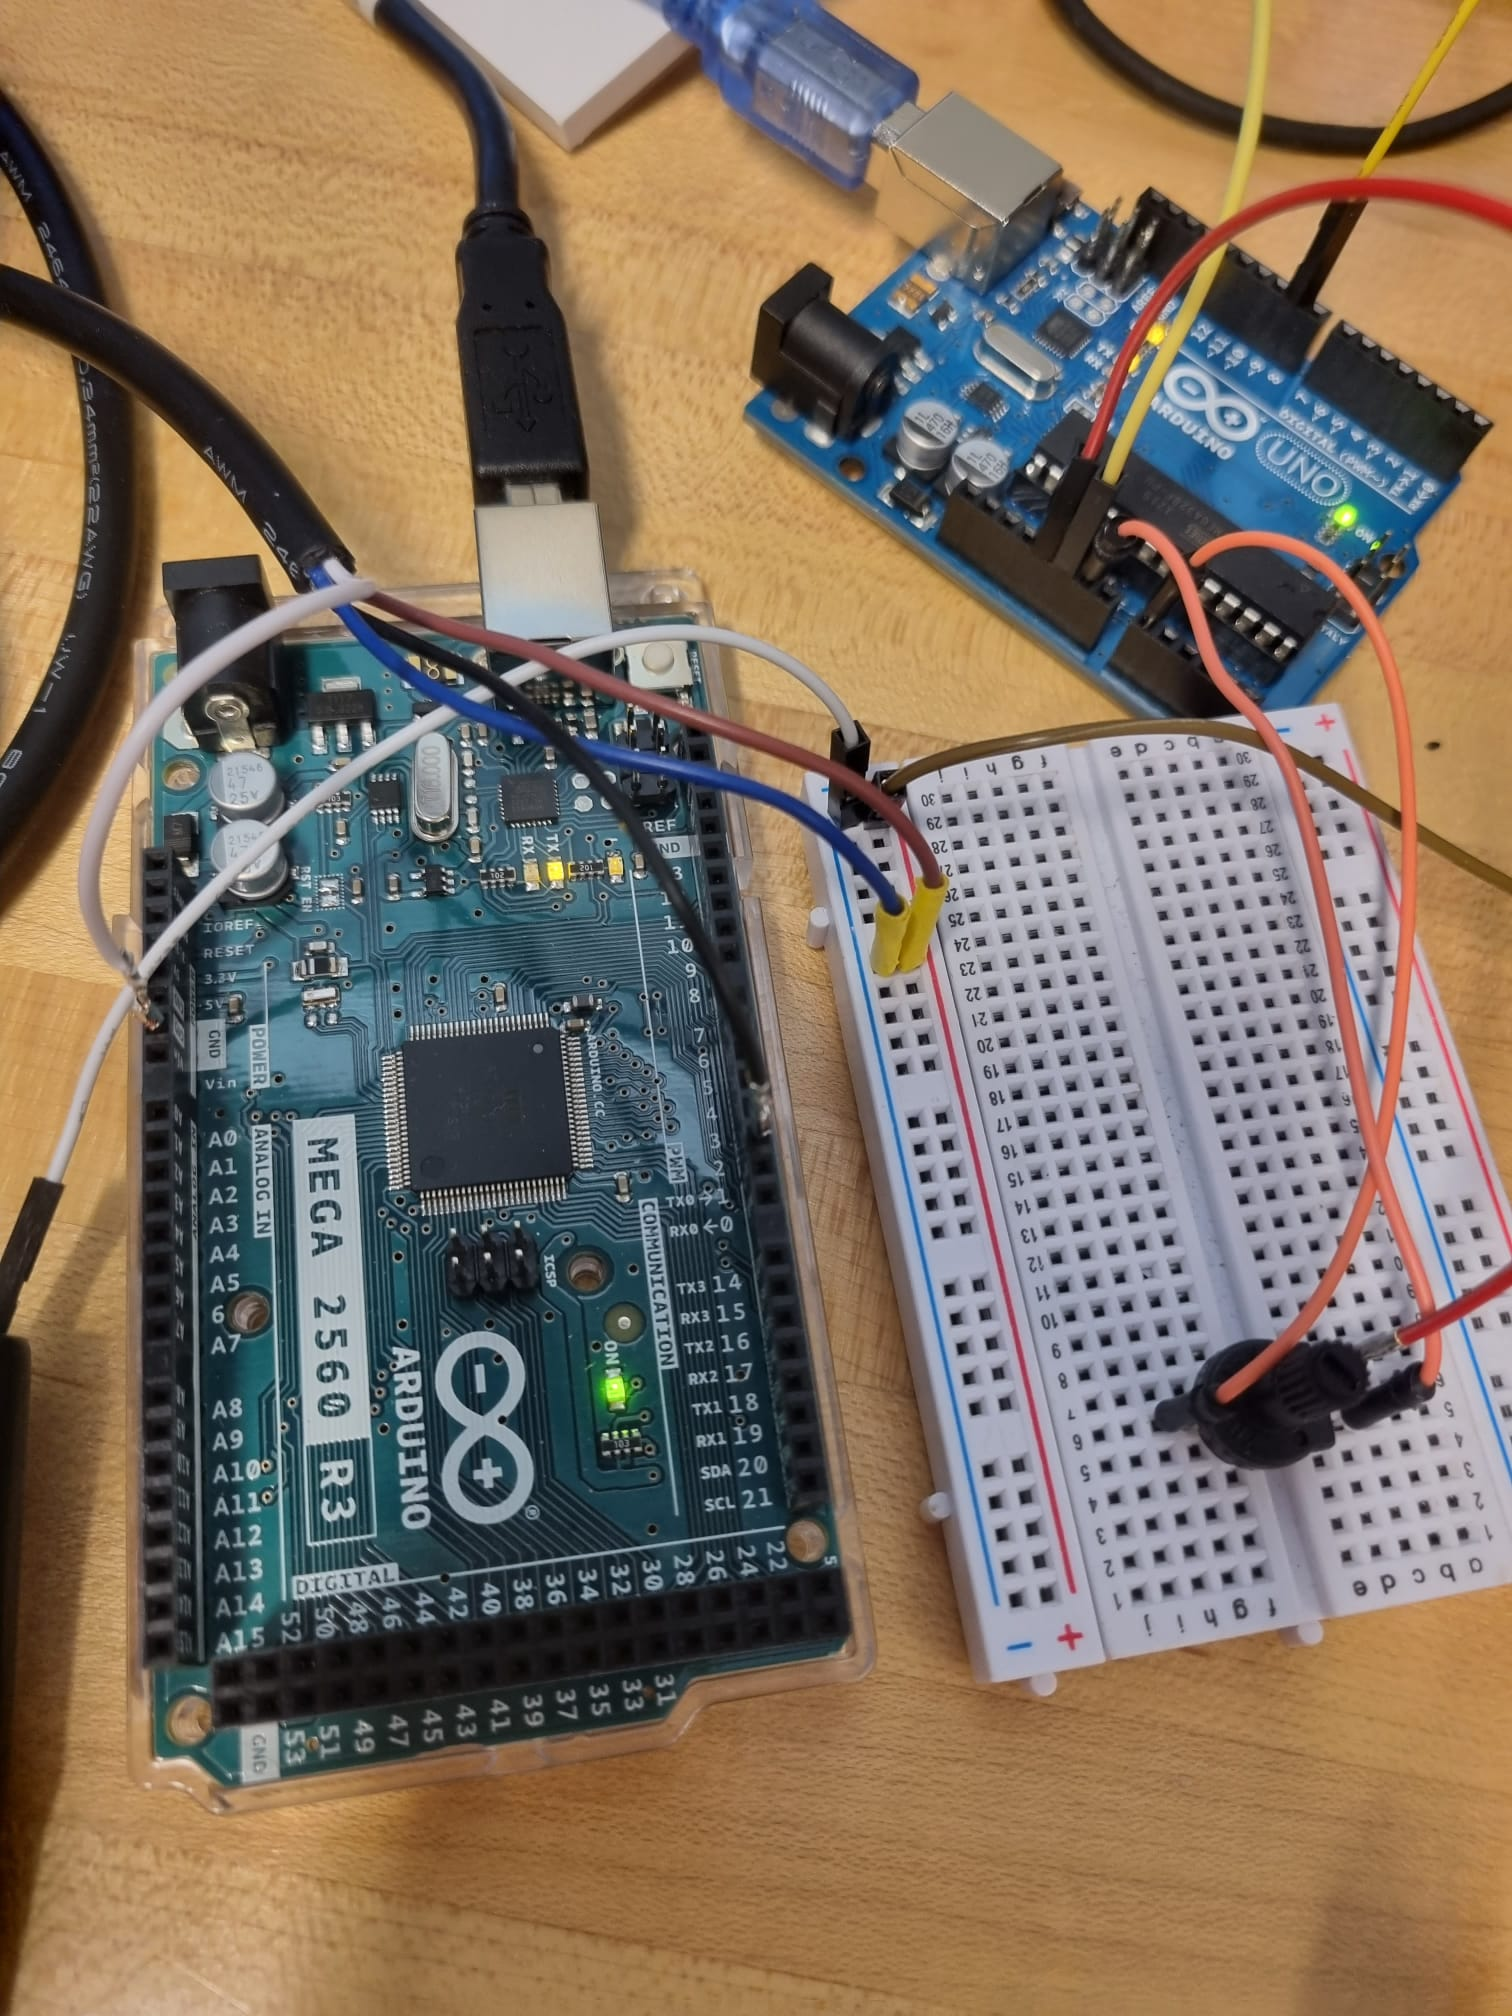
\includegraphics[width=0.5\textwidth]{arduino_tach.jpeg}
	\caption{SICK sensor digital connection to arduino mega 2560 R3}
	\label{fig:sick_arduino_digital}
\end{figure}

Specifications of these sensors can be found in this table:

\begin{table}[h!]
	\centering
	\caption{SICK WLA16 Photoelectric sensor specifications: digital output\label{tab:SICK16}}
	\begin{tabular}{||c | c ||} 
		\hline
		Output number & 2 (balck and white pins)\\ [0.5ex] 
		\hline
		Signal voltage High-Low (V) & $U_B$-2.5V / 0 (PNP) and $U_B$ / $<$ 2.5 V (NPN) \\ 
		\hline
		Output current & $\leq$ 100 mA \\
		\hline
		Switching frequency & 1000 Hz \\
		\hline
		Response time & $\leq$ 500 $\mu$s \\
		\hline
		Repeatability (response time) & 150 $\mu$s \\
		\hline
	\end{tabular}
\end{table}

A switching frequency of 1000 Hz implies that the sensor can complete 1000 readings in one second. In other words, it can read one complete measurement in one-thousandth of a second.

In the case of a quadcopter like the one intended to use in this work, the speed of the propellers stays in the range of 1000 up to 12000 revolutions per minute. Translating this numbers to revolutions per second, the range becomes 17 to 200 revolutions per second, which fits comfortably in the switching frequency of the sensors chosen.

It must be said that the switching frequecy stated in the datsheet is obtained with a light/dark ratio of 1 to 1.


\subsubsection{Codes files}
In this project, there are several arduino files that collect data from this sensor according to the connection established. Eventhoug the sensors are purely digital, the analog alternative was also tested.



The digital connection and function of 1 up to 4 sensors can be tested with the codes in the Arduino folder (tachometer\_nsensor), with \textit{n} the number of sensors willing to be connected.

\textit{tachometer\_1sensor.ino} is a script for only one sensor and uses a timer to count the time that passes in between sensor interrupts. For more information on microcontroller timers and sensor interrupts, see \autoref{sec:ontimersandinterrupts}. The same approach has been used for \textit{tachometer\_2sensor.ino}, showing that the timer system is not the best choice when dealing with more than one sensor.

\textit{tachometer\_3sensor.ino} and \textit{tachometer\_4sensor.ino} deal with three and four sensors, respectively by using only interrupts on three and four pins of the arduino Mega. This way, a delay is introduced for the counters to measure the sensor occurrences and once the delay is over, the elapsed time and counts are used to compute the RPM.


\subsection{Timers and interrupts}
\label{sec:ontimersandinterrupts}

Arduino Mega2650 R3 contains an \hyperref{https://ww1.microchip.com/downloads/en/devicedoc/atmel-2549-8-bit-avr-microcontroller-atmega640-1280-1281-2560-2561_datasheet.pdf}{category}{name}{ATMEGA2650 microcontroller}, and a 16 MHz oscillator.

\begin{figure}[h!]
	\centering
	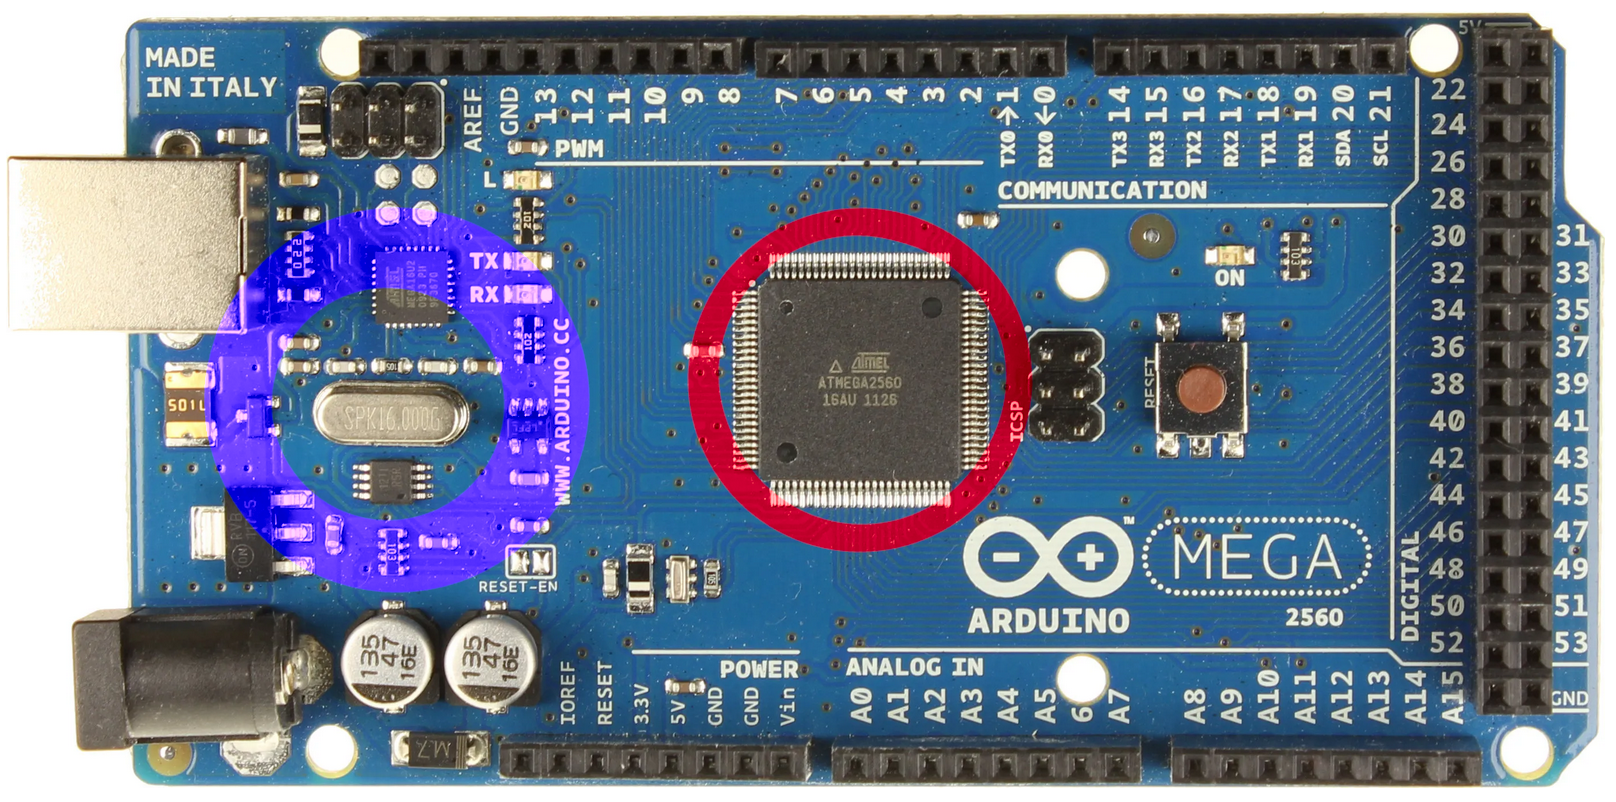
\includegraphics[width=0.5\textwidth]{arduino_mega.png}
	\caption{Arduino mega2650, the oscillator is in the blue circle and the microcontroller is in the red one}
	\label{fig:arduino_mega}
\end{figure}

\textbf{Waveform Generation mode} or WGMn3:0 bits located in the Timer/Control regsiters A and B. (from page 139 of the manual) determines the counting sequence. When setting TCCR1A and TCCR1B to 0, we are choosing the \textit{normal} mode, in which the counting direction is always incremented and no counter clear is implemented.  The counter simply overruns when passes its maximum 16-bit value and then restarts from the bottom. In the case of a 16 it counter, we have the following:

\begin{equation}
	Steps = 2^{16bits} = 65536
\end{equation}

The oscillator of the board can process 16000000 steps in one second, so our counter runs into an overflow every:

\begin{equation}
	\frac{65536 steps}{16e10^{6}\frac{steps}{second}} \approx 4ms
\end{equation}

The following figure represents the counter behavior with a waveform generator in normal mode and a prescaler of 1.

\begin{figure}[h!]
	\centering
	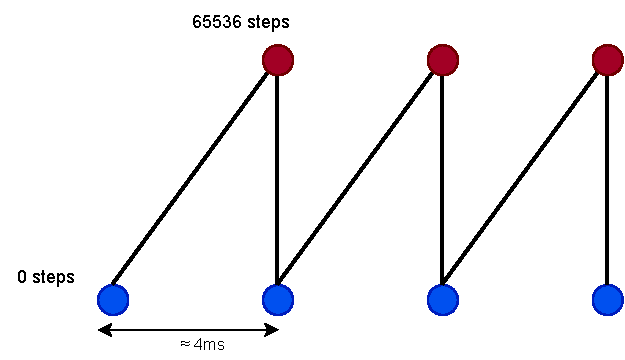
\includegraphics[width=0.6\textwidth]{Counter.pdf}
	\caption{Counter overflow process}
	\label{fig:counter}
\end{figure}

A prescaler is a number used to control the overflow frequency of a  counter. If the prescaler is set to 1, this means that the equation above is going to rule out counter overflow.

We can enable the counter overflow interrupt by setting the TOIE1 bit to 1. This allows us to construct an interrupt that is triggered every time the counter overflows. The prescaler of timer 1 (CS1n with n from 0 to 2) acts as follows:

\begin{equation}
	\frac{65536 [steps]}{16\cdot10^{6}/prescaler[\frac{steps}{second}]}
\end{equation}

The table with values of the prescaler and the bits to be set is the following:

\begin{figure}[h!]
	\centering
	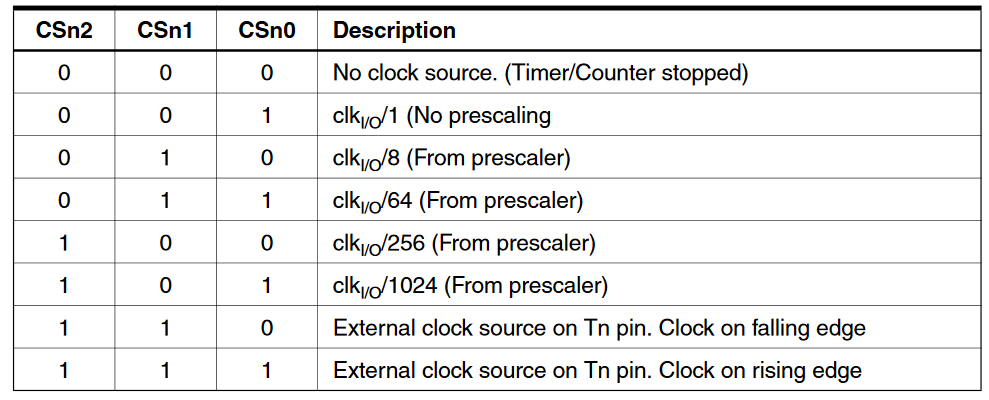
\includegraphics[width = 0.6\textwidth]{CSn.png}
	\caption{Clock select bit description}
	\label{fig:CSn}
\end{figure}

This means that the minimum interrupt frequency we can obtain with a 16-bit counter is around 4 milliseconds. 


There's other two ways of controlling counter overflow frequency:

\begin{itemize}
	\item Start the counter at a different value than 0. Refer to \autoref{eq:formula1} to figure out how to compute the starting point
	\item Use clear timer on compare match. This mode can be activated by setting WGM12 to 1. It allows the user to manipulate the counter resolution by comparing the counter value to a pre-established value.
\end{itemize}


\begin{equation}
	Start = 65536 - \frac{f_{clock}}{Prescaler\cdot f_{target}}
	\label{eq:formula1}
\end{equation}


In the case of building a tachometer with a digital sensor, this \hyperref{https://www.youtube.com/watch?v=6QZMt4yyylU}{category}{name}{video} has been used as inspiration, changing the value of the oscillator.

In our case, using a prescaler of 256 allows us to reduce the counter maximum to 62500 (from $2^{16}$ to $2^{16}/256$).
In this case, the time it takes for one revolution to complete can be described as:

\begin{equation}
	\frac{counter [\frac{steps}{1rotation}]}{62500 [\frac{steps}{1second}]}
\end{equation} 

To obtain the RPM value:

\begin{equation}
	\frac{60seconds}{1minute}\cdot\frac{62500 [\frac{steps}{1second}]}{counter [\frac{steps}{1rotation}]}
\end{equation}

Depending on the value of the counter when entering the interrupt we can get a hypothetical maximum of 3750000 RPM and a minimum of 57 RPM.

\subsection{Only interrupt based algorithms (FINAL CHOICE)}

In the end, the use of timers to control 4 tachometers is becoming a very tedious task and readings are not correct. The final solution that was adopted is the use of four interrupts attached to the interrupt enabled pins of the arduino Mega 2650 R3 (2, 3, 18, 19, 20, 21 (pins 20 \& 21 are not available to use for interrupts while they are used for I2C communication)). Increasing four counters and computing the rpm every loop iteration allows the control of the resolution and maximum and minimum values to be captured with the sensors.

The algorithm is as follows:

\begin{algorithm}
	\begin{algorithmic}
		\Ensure Interrupt pins: 2, 3, 18, 19 and Serial communication open
		\State $delay \gets 2000ms$
		\State $X \gets x$
		\State $N \gets n$
		\While{$Working$}
		\For{$t = 0$ to $t = delay$}
		\State $counter_1  ++ $
		\State $counter_2  ++ $  
		\State $counter_3  ++ $
		\State $counter_4  ++ $
		\EndFor
		\\Stop all interrupts 
		\State $t \gets Update  $
		\State $rpm1 \gets 60000\frac{ms}{1min} \times \frac{counter_1}{t_{elapsed}} $
		\State $rpm2 \gets 60000\frac{ms}{1min} \times \frac{counter_2}{t_{elapsed}} $
		\State $rpm3 \gets 60000\frac{ms}{1min} \times \frac{counter_3}{t_{elapsed}} $
		\State $rpm4 \gets 60000\frac{ms}{1min} \times \frac{counter_4}{t_{elapsed}} $
		\State $counter_1  \gets 0 $
		\State $counter_2  \gets 0$  
		\State $counter_3  \gets 0 $
		\State $counter_4  \gets 0 $
		\EndWhile
	\end{algorithmic}
\caption{An algorithm with caption}
\label{alg:cap}
\end{algorithm}

The resolution of the readings depends on the product of $60000\frac{ms}{1min} \times \frac{1}{t_{elapsed}}$. Depending on the delay imposed, the resolution will change. Also, the minimum and maximum values to be read will be different.


The Arduino counters have been defined as \textit{volatile}\cite{volatiles} floats, which is directing the compiler to load the variable from RAM and not from a storage register. Values stored in registers can be inaccurate under certain conditions. Variables such as counters inside interrupts are being changed by something beyond the control of the code section (setup or loop code). Declaring them as \textit{volatile}, the changes in them are immediately visible in the \textit{loop()} function. If not, the variable state might be loaded int o a register when entering the function and would not be updated anymore until the function ends. 
Declaring a variable \textit{volatile} is a directive to the compiler.


\section{Castle Phoenix Edge 50A ESC}
\label{sec:ESC}
The manual of these ESC is in the following \hyperref{https://dzf8vqv24eqhg.cloudfront.net/userfiles/4671/6540/ckfinder/files/Product%20Manuals/Aircraft%20Helis/Phoenix%20Edge%20Series/edge_guide.pdf?Policy=eyJTdGF0ZW1lbnQiOlt7IlJlc291cmNlIjoiaHR0cHM6Ly9kemY4dnF2MjRlcWhnLmNsb3VkZnJvbnQubmV0L3VzZXJmaWxlcy80NjcxLzY1NDAvY2tmaW5kZXIvZmlsZXMvUHJvZHVjdCUyME1hbnVhbHMvQWlyY3JhZnQlMjBIZWxpcy9QaG9lbml4JTIwRWRnZSUyMFNlcmllcy9lZGdlX2d1aWRlLnBkZiIsIkNvbmRpdGlvbiI6eyJEYXRlTGVzc1RoYW4iOnsiQVdTOkVwb2NoVGltZSI6MTY5MjExNDY5OX19fV19&Signature=Ttin0Hxd-W1Av7ACk8UNA7CYOoaI9~KpY5-N3fKi5dI-KHRJRYZSGEDBNtASKJYoFXJGzLuWZmpiy5EDsTr-ZWxcN2yKQiWBwiXAG5Ntc3~4cLVdHm6XacfGUEBSlxb20EiOOYZ8MGA5RKDY~8~ws85YxoU8X4pa79NiWuHGlPQ4phsYztgbzeIrGpJSADMONCXLsvYziu1AHUeHOdPgZNyapAdTpVS85KuHCU7op72VtraeqWH9zaRxO6dwdQxqBsx3qs18JsE3f4ET3khM7HGiHr6H9p5j-l0ij8cLhZET0bTB7Hqlwe95accVxRQzJJ4EjaYpaK0CzYUycD~RwA__&Key-Pair-Id=K2TK3EG287XSFC}{category}{name}{link}.

The programming instructions were followed to obtain the following configuration:

\begin{itemize}
	\item Settings 1: Option 4. 3.3V per cell
	\item Settings 2: Option 5. Brake Disabled (Factory Settings)
	\item Settings 3: Option 3: RPM Decrease
	\item Settings 4: Option 2: 12 kHz (Factory Settings)
\end{itemize}

Tho enter programming mode either follow the instructions on the manual or follow the next steps:

\begin{itemize}
	\item Unplug your ESC and select full throttle with your transmitter
	\item Plug your ESC and wait for 5 seconds or so. You will hear a song, two beeps and the same song again. Take your throttle to medium position and wait for the song again.
	\item Once you've heard the song, go back to full throttle and wait for another confirmation with the same song. Then go back to half throttle. 
	\item If at this point you should hear the song repeat itself four times. Then your have entered programming mode.
	\item The options will be introduced to you as a first \textit{beep} sequence indicating the setting number and a second \textit{beep} sequence indicating the option number. By moving the throttle to maximum position, we are accepting the option in this setting number. If accepted, the ESC will pass onto the next setting number. If rejected by taking the throttle to the minimum, the ESC will ask about the next option in the same setting number.
	To let us know that the ESC has understood our command, it will start emitting two beeps at a faster rate. move the throttle stick to middle position to pass onto the next setting/option query. 
\end{itemize}

The ESC connection to the arduino is shown in \autoref{fig:arduino_ESC}:

\begin{figure}[h!]
	\centering
	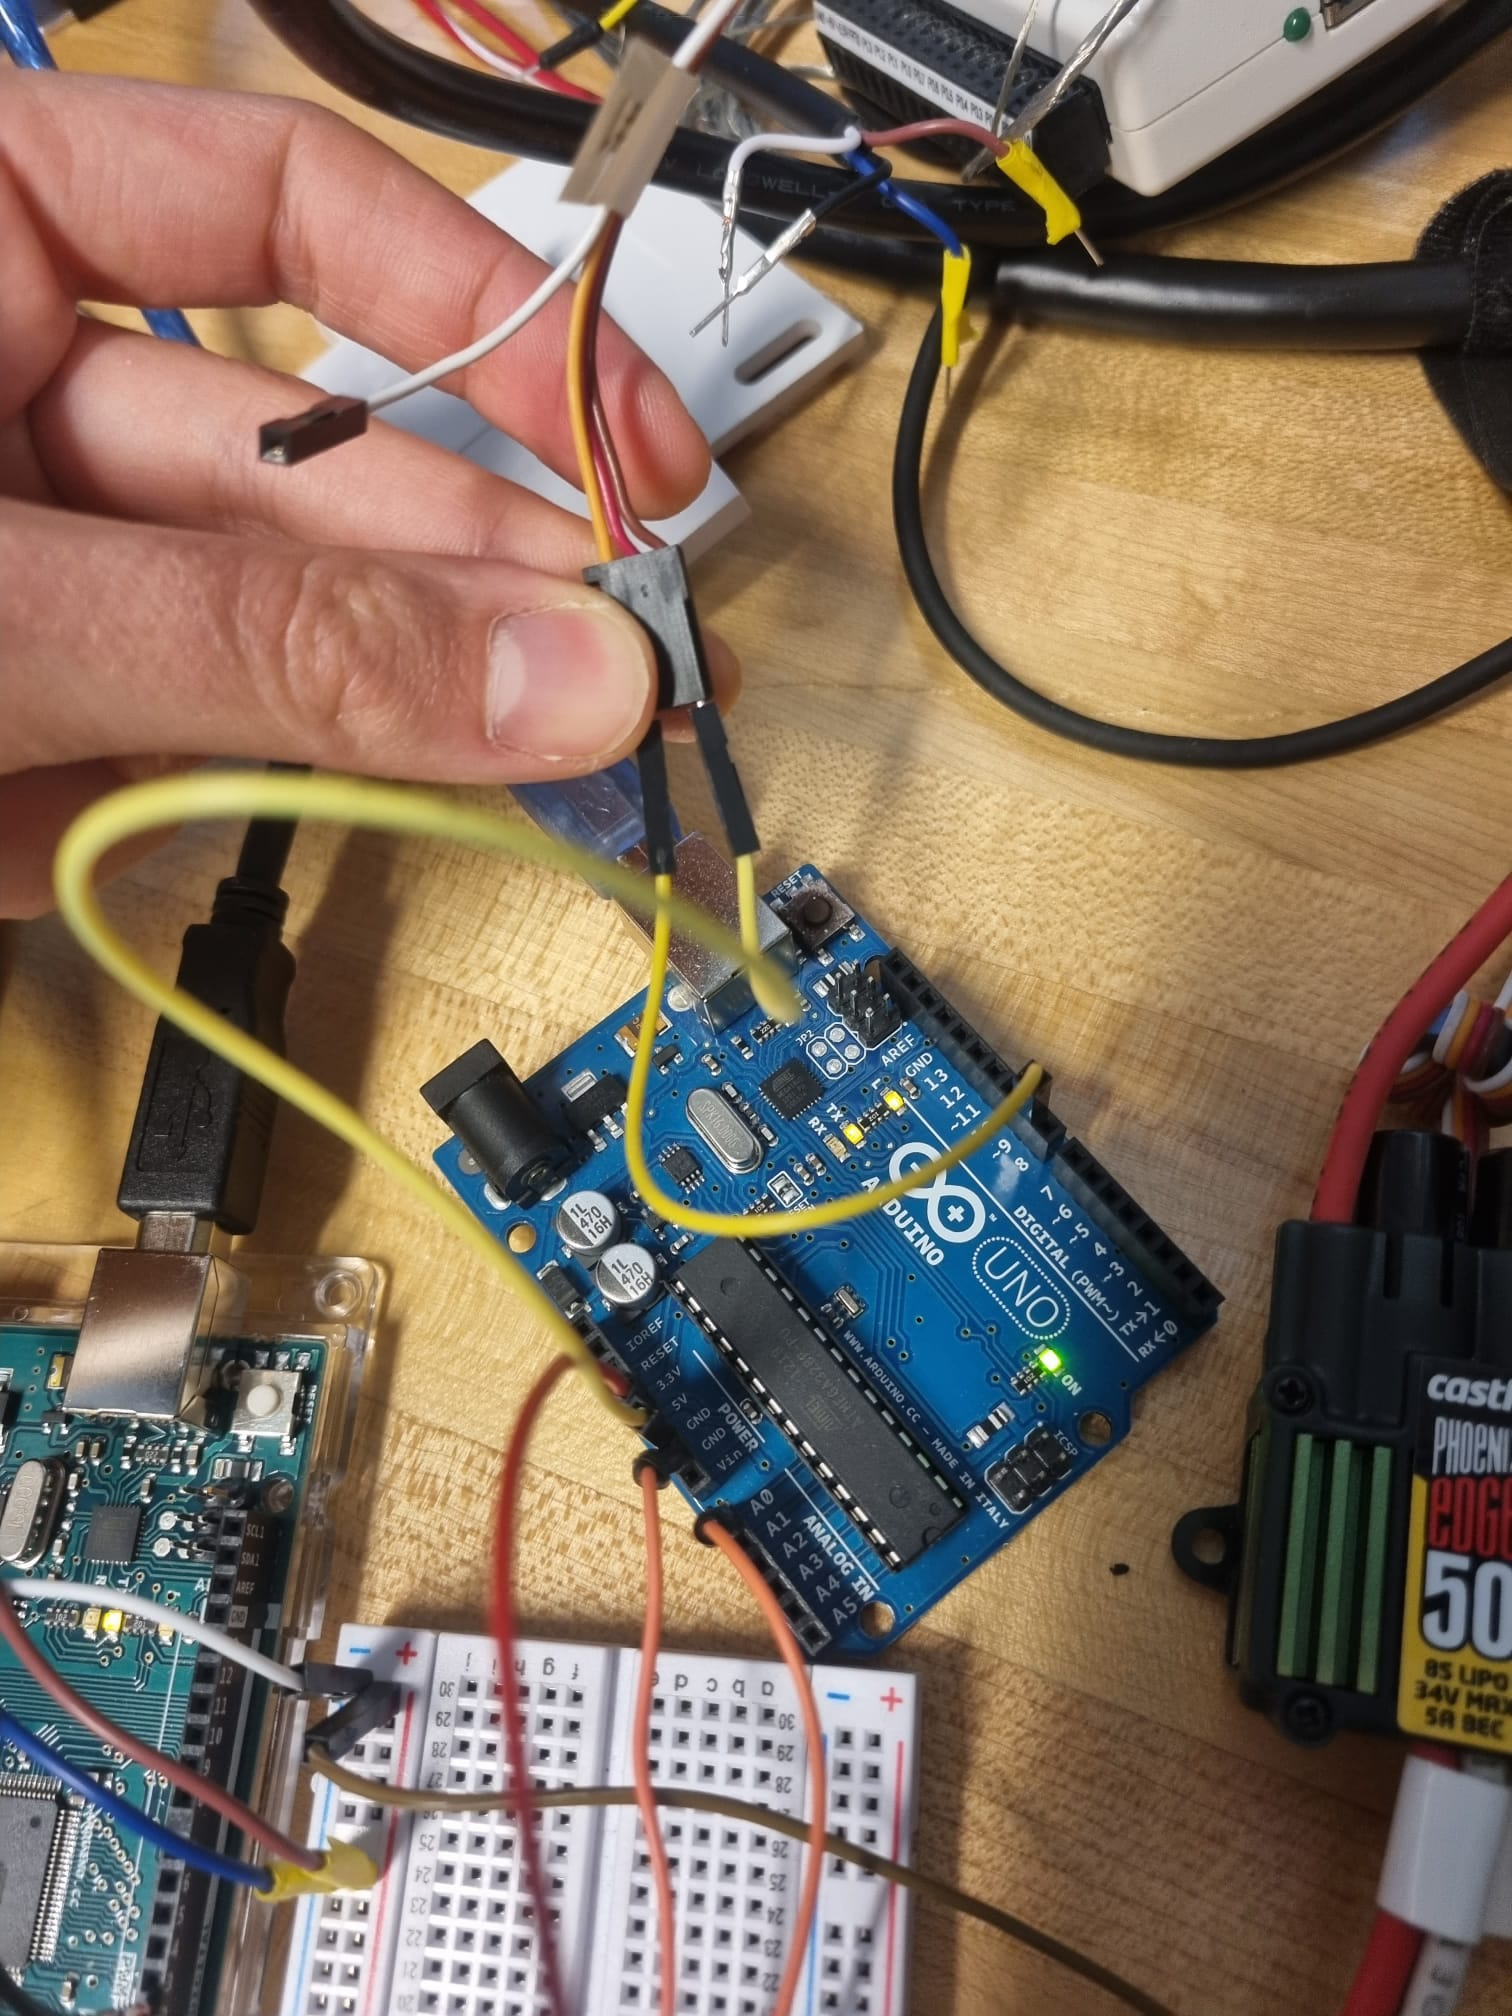
\includegraphics[width=0.5\textwidth]{arduino_ESC.jpeg}
	\caption{Brown ESC wire connects to GND and orange ESC wire is attached to pin 9 for PWM signal}
	\label{fig:arduino_ESC}
\end{figure}

The rest of the cables are connected to a potentiometer that acts as radio controller.




\section{The quadcopter}

The quadcopter used in the ground/ceiling/wall effect tests is depicted in figure ??? and is constituted by a metallic frame that enables different distancing between the motors. The ESC are the ones discussed in \autoref{sec:ESC}, which can be powered by a 2s LiPo battery (7.4 V) up to an 8s (33.6 V). These controllers draw a maximum of 50 A at full throttle.

More than one motor type is used since different propeller sizes are tested trying to stay close to a ratio of 2 between the diameter and the pitch. The propsed propellers are the following:

\begin{itemize}
	\item 9" x 4.7" (Ratio = 1.92)
	\item 10" x 4.5" (Ratio = 2.22)
	\item 12" x 6" (Ratio = 2)
	\item 13" x 6.5" (Ratio = 2)
	\item 15" x 5.5" (Ratio = 2.72)
\end{itemize}




\section{Power supply}

The system needs more than one source of power to feed the boards and the sensors. 

The Arduinos are powered with a PC, while the sensors require a higher voltage and current.

The tachometers are powered by a switching adapter that provides 12 V and a maximum of 500 mA which is a suitable option since the current draw of these devices is not very high.

The force/torque sensor is powered by its own black box. Please, refer to page 13 from the \hyperref{https://www.ati-ia.com/app_content/documents/9620-05-DAQ.pdf}{category}{name}{manual} for more information regarding powering this component.

The quadcopter is powered with two Astec DS550-3 power supplies connected in parallel using active load sharing. This way, a stable 12V and 90A (max) can be provided to the quadcopter, granting the repeatability of the experiments.

\section{The final architecture}

\begin{figure}[h!]
	\centering
	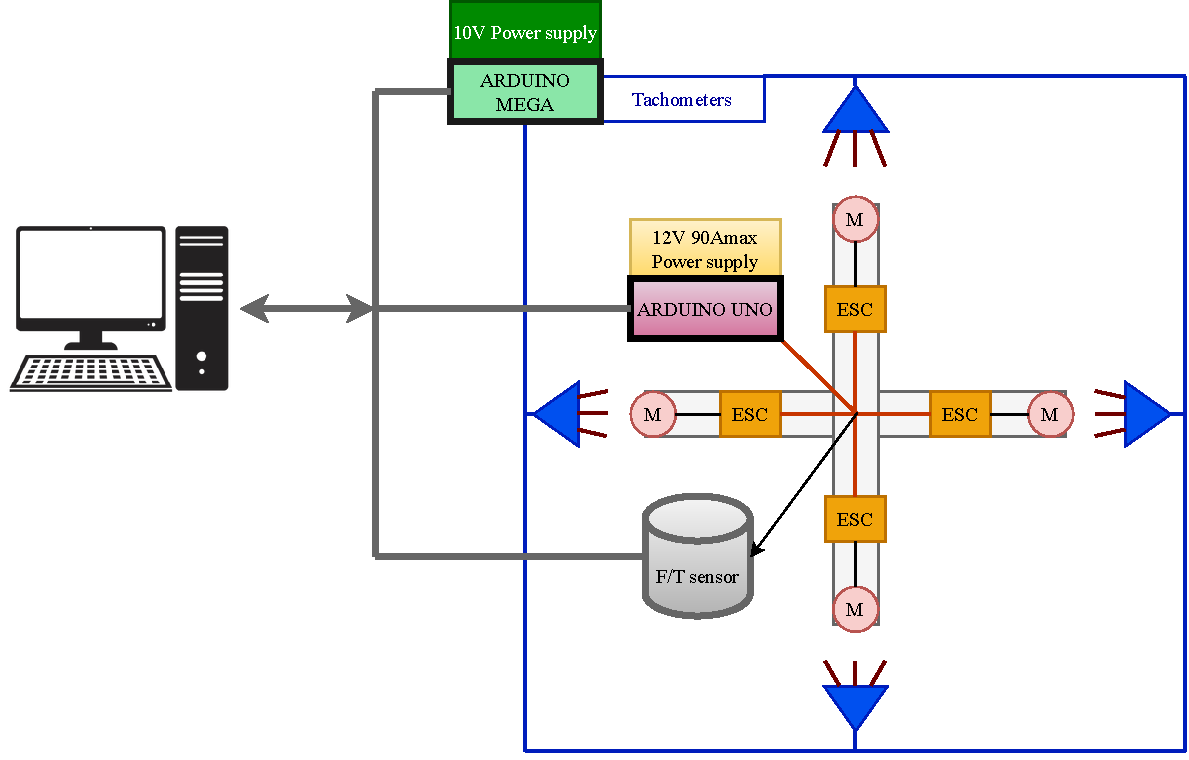
\includegraphics[width=0.9\textwidth]{General_setup.pdf}
	\caption{A graph of the overall system, representing all devices and the connections between them}
	\label{fig:overall_system}
\end{figure}

\subsection{Data collection procedure}






\section{Resources}

\href{https://documentation.help/Keysight-34970A-34972A/documentation.pdf}{Keysight 34970A/34972A Command Reference Manual}

\bibliographystyle{IEEEtran}
\bibliography{biblio}

\end{document}
